%% Template 
%% credits: Prof. William D'Andrea Fonseca - Eng. Acústica UFSM 
%% (adapted by Sergio Aguirre) 
%%%%%%%%%%%%%%%%%%%%%%%%%%%%%%%%%%%%%%%%%%%%%%%%%%%%%%%%%%%%%%%%%%%%%%%%%%%%%%%%%%%%%%%%%%%%%%%%%%%%%%%%
\documentclass[12pt, a4paper, twoside, onecolumn]{article}%
%%%%%%%%%%%%%%%%%%%%%%%%%%%%%%%%%%%%%%%%%%%%%%%%%%%%
%%% Linguagem e entrada
\usepackage[utf8]{inputenc} 
\usepackage[english]{babel}
\usepackage[T1]{fontenc}
\usepackage{mathptmx} 
\usepackage{enumitem}
\usepackage{units}
%%%%%%%%%%%%%%%%%%%%%%%%%%%%%%%%%%%%%%%%%%%%%%%%%%%%
\usepackage{HEAR2018} %%% Basic template settings
%%%%%%%%%%%%%%%%%%%%%%%%%%%%%%%%%%%%%%%%%%%%%%%%%%%%
\usepackage{HEARopts} %%% Package with additional and optional configurations
%%%%%%%%%%%%%%%%%%%%%%%%%%%%%%%%%%%%%%%%%%%%%%%%%%%%
\usepackage{xargs} % Use more than one optional parameter in a new commands
% \usepackage{fancyhdr}
% \usepackage{hyperref}
% \usepackage{BackrefEN}
\usepackage{multirow}
\usepackage{graphicx}
%\usepackage[table,xcdraw]{xcolor}


%%%%%%%%%%%%%%%%%%% set comments %%%%%%%%%%%%%%%%%%%%%%%%%%%%%%%%
\usepackage[colorinlistoftodos,prependcaption,textsize=footnotesize]{todonotes}
\newcommandx{\unsure}[2][1=]{\todo[linecolor=red,backgroundcolor=red!25,bordercolor=red,#1]{#2}}
\newcommandx{\change}[2][1=]{\todo[linecolor=blue,backgroundcolor=blue!25,bordercolor=blue,#1]{#2}}
\newcommandx{\info}[2][1=]{\todo[linecolor=OliveGreen,backgroundcolor=OliveGreen!25,bordercolor=OliveGreen,#1]{#2}}
\newcommandx{\improvement}[2][1=]{\todo[linecolor=Plum,backgroundcolor=Plum!25,bordercolor=Plum,#1]{#2}}
\newcommandx{\thiswillnotshow}[2][1=]{\todo[disable,#1]{#2}}
\newcommand{\note}[1]{\todo[inline]{#1}}
%%%%%%%%%%%%%%%%%%%%%%%%%%%%%%%%%%%%%%%%%%%%

\pagestyle{fancy} 
\fancyhf{{\rule[-0.4em]{1\linewidth}{.3pt}}}
\fancyhead[LO]{\nouppercase{\textsf{\rightmark}}}
\fancyhead[LE]{\nouppercase{\textsf{\rightmark}}}
\fancyhead[RE]{\thepage}
\fancyhead[RO]{\thepage}
\fancyfoot[RO]{\vspace{2.5mm}\footnotesize{ERH}}
\fancyfoot[LE]{\vspace{2.5mm}\footnotesize{}}
\cfoot{}
%\fancyfoot[LO]{{\rule[0.1em]{1\linewidth}{.2pt}}\hfill
\includegraphics[height=0.45cm]{Config/HEAR2.png}}
%\fancyfoot[RE]{{\rule[0.1em]{1\linewidth}{.2pt}}\hfill
\includegraphics[height=0.45cm]{Config/HEAR2.png}}

%%%%%%%%%%%%%%%%%%%%%%%%%%%%%%%%%%%%%%%%%%%%%%%%%%%%
\hypersetup{
  pdfinfo={
	 Subject={Objectives},
   Keywords={Studies, Objectives}
  }
}

\usepackage{Codes2Latex}
%% Pre−load languages
\lstloadlanguages{WMatlab,WFortran,WLatex,WLabview,ttcCode}

\usepackage{background}
\backgroundsetup{
  position=current page.east,
  angle=-90,
  nodeanchor=east,
  vshift=-2.5mm,
  opacity=.8,
  scale=3,
  contents=Draft
}


%\usepackage{lineno} \linenumbers %%% Ative para numerar as linhas
%%%%%%%%%%%%%%%%%%%%%%%%%%%%%%%%%%%%%%%%%%%%%%%%%%%%%%%%%%%%%%%%%%

\begin{document} 
%%%%%%%%%%%%%%%%%%%%%%%%%%%%%%%%%%%%%%%%
%% Cover 
%%%%%%%%%%%%%%%%%%%%%%%%%%%%%%%%%%%%%%%%

\newgeometry{left=0cm,right=0cm,top=0cm,bottom=0cm}

\thispagestyle{empty}

\begin{titlepage}

\begin{figure}[ht]
\begin{minipage}{.12\textwidth}
%%%%%%%%%%%%%%%%%%%%%%%%%%%%%%%%%%%%%%%%%%%%%%%%%%%%%%%%%%%%%%%%%%%%%%%%%%	
%%%%%%%%%%%%%%%%%%%%%%%%%%%%%%%%%%%%%%%%%%%%%%%%%%%%%%%%%%%%%%%%%%%%%%%%%%
%%% Edit here the COLOR of the side box
\colorbox{bhear}    % 
	{
	\begin{minipage}[c]{.9\textwidth}
	\vspace{299mm}
 	$\,$ 
	\end{minipage}
	}
\end{minipage}
\hfill
\begin{minipage}{.83\textwidth}
%%%%%%%%%%%%%%%%%%%%%%%%%%%%%%%%%%%%%%%%%%%%%%%%%%%%%%%%%%%%%%%%%%%%%%%%%%	
%%% Edit here the header	
	
\begin{center}
{\rule[1.1em]{.9\linewidth}{.1pt}}\hfill
     ITA-Toolbox initial 
{\rule[0.1em]{.9\linewidth}{.1pt}}\hfill
\end{center}
	

	
%%%%%%%%%%%%%%%%%%%%%%%%%%%%%%%%%%%%%%%%%%%%%%%%%%%%%%%%%%%%%%%%%%%%%%%%%%	
  \begin{minipage}[t]{1\linewidth}
		\sffamily
%%%%%%%%%%%%%%%%%%%%%%%%%%%%%%%%%%%%%%%%%%%%%%%%%%%%%%%%%%%%%%%%%%%%%%%%%%
%%%%%%%%%%%%%%%%%%%%%%%%%%%%%%%%%%%%%%%%%%%%%%%%%%%%%%%%%%%%%%%%%%%%%%%%%%		
%%% Edit here the text
		%\vspace{1cm}
\hspace{.7cm}	%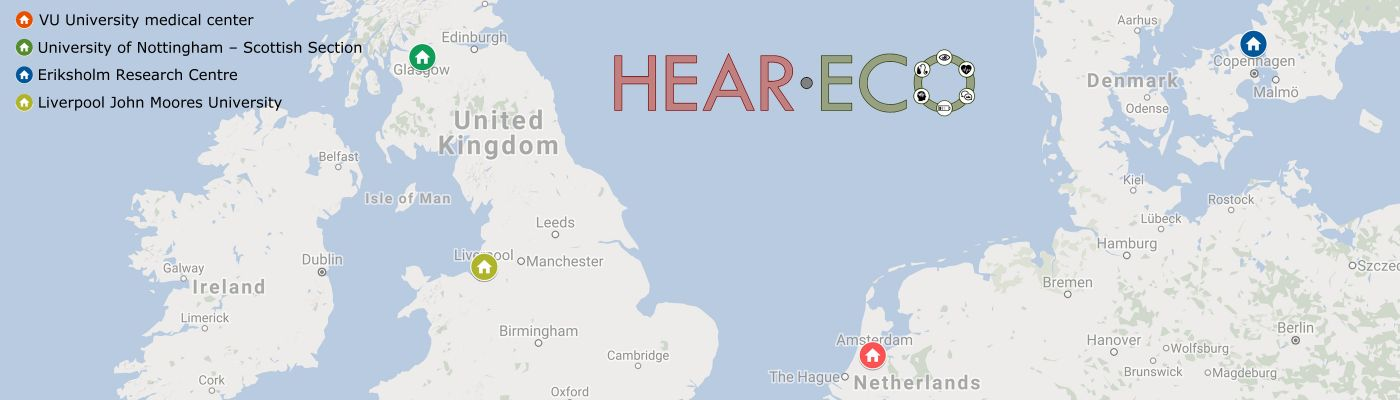
\includegraphics[width=.60\linewidth]{Config/places.jpg}\qquad
\includegraphics[width=.256\linewidth]{Config/flag.jpg}


		%\Huge Explorative Studies in New Biomarkers\\ of Listening Effort and Motivation
		
	\vspace{2cm}
% 		\Large{\textbf{ESR 6 }} %First Year Plan
	\vspace{.4cm}
	
% 		\large{\textit{Experiment 2 Plan}}
		\vspace{2cm}
		


% {\fontsize{12}{15}\selectfont Aguirre, Sergio L.; Whitmer, William; Lunner, Thomas}

\vspace{0.5cm}

% {\fontsize{8}{13} \selectfont (1)\,Medical Research Council/Chief Scientist Office Institute of Hearing Research - Scottish Section, Glasgow-UK.\\(2)\,Cognitive Hearing Science, Linnaeus Centre HEAD Department of Behavioural Sciences and Learning\\Linköping University Sweden. Hearing Systems, Department of Electrical Engineering - Technical University of Denmark.\\[2pt]\par}

%\scriptsize{(1)~Medical Research Council/Chief Scientist Office Institute of Hearing Research - Scottish Section, Glasgow-UK.\\(2)~ Cognitive Hearing Science, Linnaeus Centre HEAD Department of Behavioural Sciences and Learning\\Linköping University Sweden. Hearing Systems, Department of Electrical Engineering - Technical University of Denmark.}


\vspace{10cm}
% \footnotesize{This project has received funding from the European Union’s Horizon 2020 research and\\innovation programme under the Marie-Sklodowska-Curie grant agreement N$^\circ$ 765329.}

\vspace{1cm}
			
		Version: $\alpha_{0.1}$
		
			\today \\
			\url{http://ita-toolbox.org/download.php}\\
			\url{https://git.rwth-aachen.de/ita/toolbox}
\end{minipage}
\end{minipage}
\end{figure}	
\end{titlepage}
\restoregeometry
\setcounter{page}{1}

% \cleardoublepage
% \phantomsection
% \tableofcontents
% \hfill\vfill
% \addtocontents{toc}{~\hfill\textbf{Page}\par}


% \cleardoublepage
% \phantomsection
% \listoffigures

% \cleardoublepage
% \phantomsection
% \listoftables

%\cleardoublepage
%\phantomsection
%%\addcontentsline{toc}{section}{List of Codes}   % English



\pagebreak
\begin{itemize}
    \item run ita\_toolbox\_setup
\end{itemize}

\begin{figure}[H]\centering
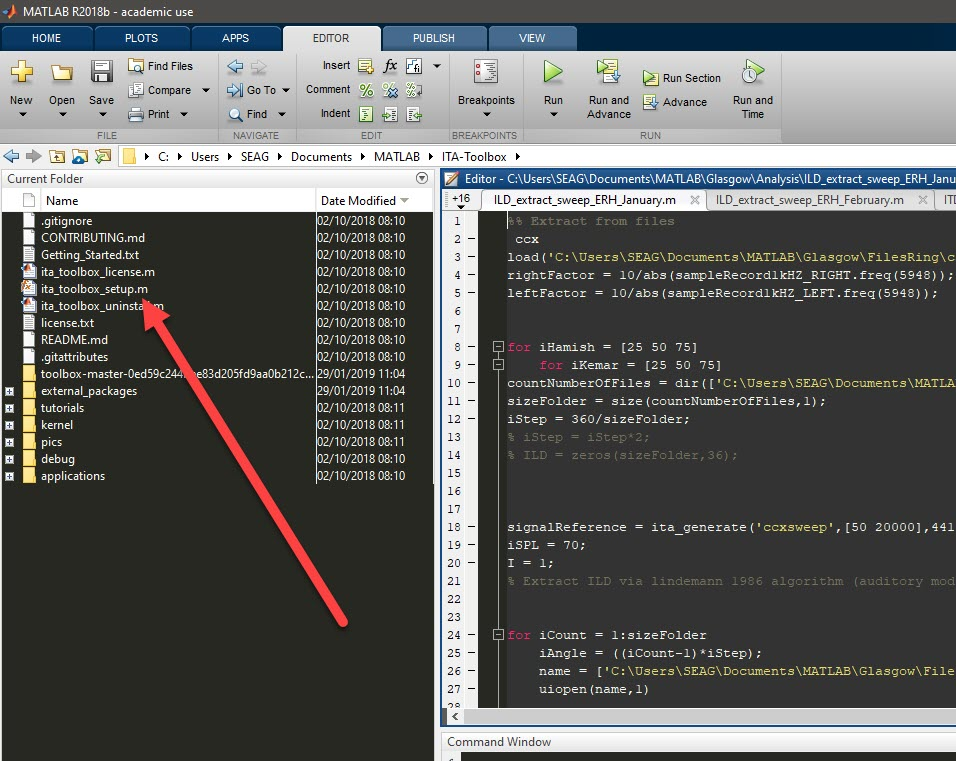
\includegraphics[width=.7\textwidth]{Figures/f1.jpg}
\end{figure}

\begin{itemize}
    \item configure your sound card and preferences
\end{itemize}

\begin{figure}[H]\centering
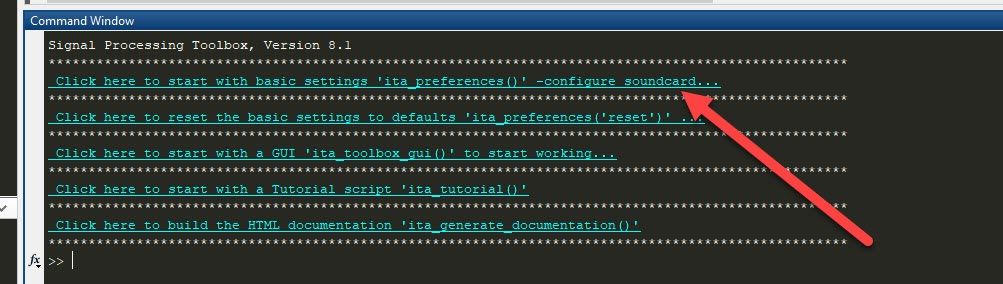
\includegraphics[width=.7\textwidth]{Figures/f2.jpg}
\end{figure}

\begin{itemize}
    \item you can access the preferences at any time using ita\_preferences
\end{itemize}

\begin{figure}[H]\centering
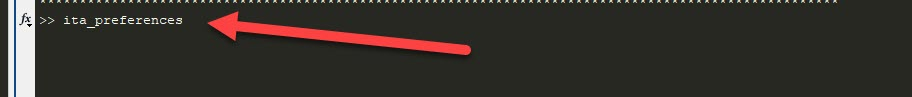
\includegraphics[width=.7\textwidth]{Figures/f3.jpg}
\end{figure}
\pagebreak

\begin{itemize}
    \item General settings
\end{itemize}
\begin{figure}[H] \centering
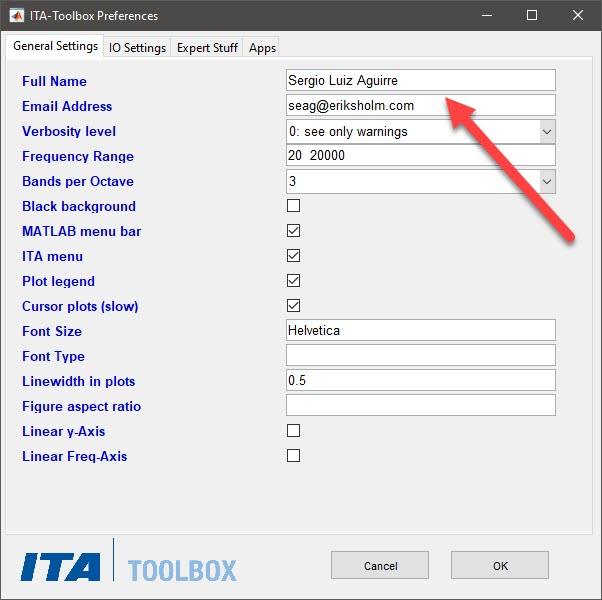
\includegraphics[width=.5\textwidth]{Figures/f4.jpg}
\end{figure}

\begin{itemize}
    \item IO settings
    \begin{itemize}
        \item  Set the driver (ASIO in this case)
    \end{itemize}
\end{itemize}

\begin{figure}[H] \centering
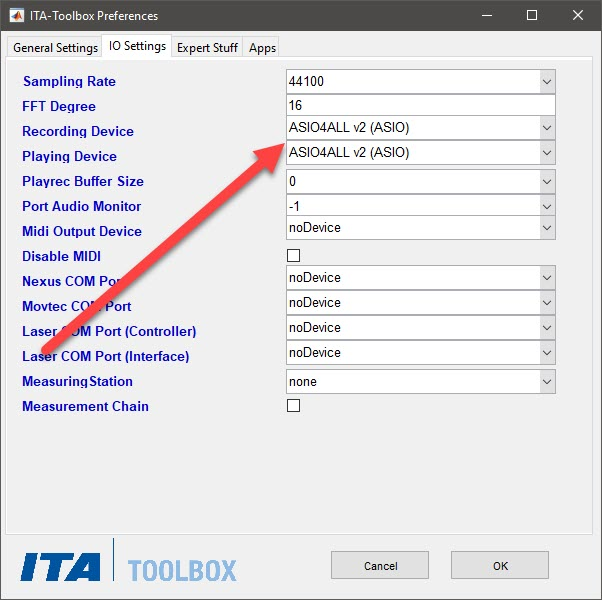
\includegraphics[width=.5\textwidth]{Figures/f5.jpg}
\end{figure}
\vfill

\pagebreak
\begin{itemize}
    \item Port Audio Monitor (Change to 1 to get the level meter and stop button) 
\end{itemize}

\begin{figure}[H] \centering
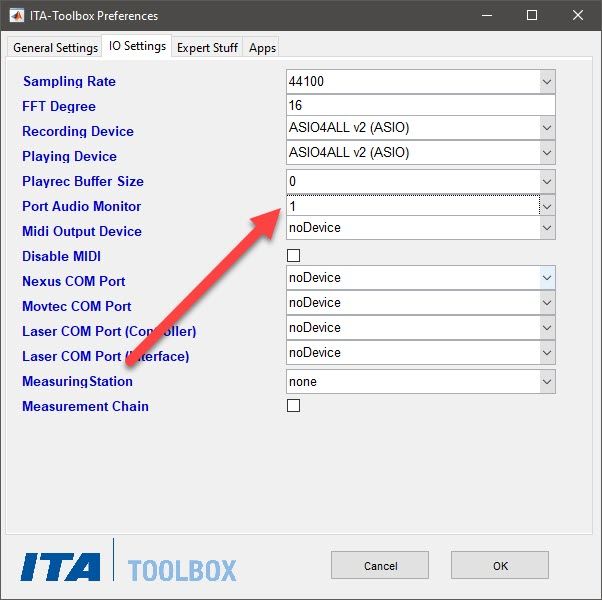
\includegraphics[width=.5\textwidth]{Figures/f6.jpg}
\end{figure}



\begin{itemize}
    \item after itaObject ``.tab'' present the options
\end{itemize}

\begin{figure}[H] \centering
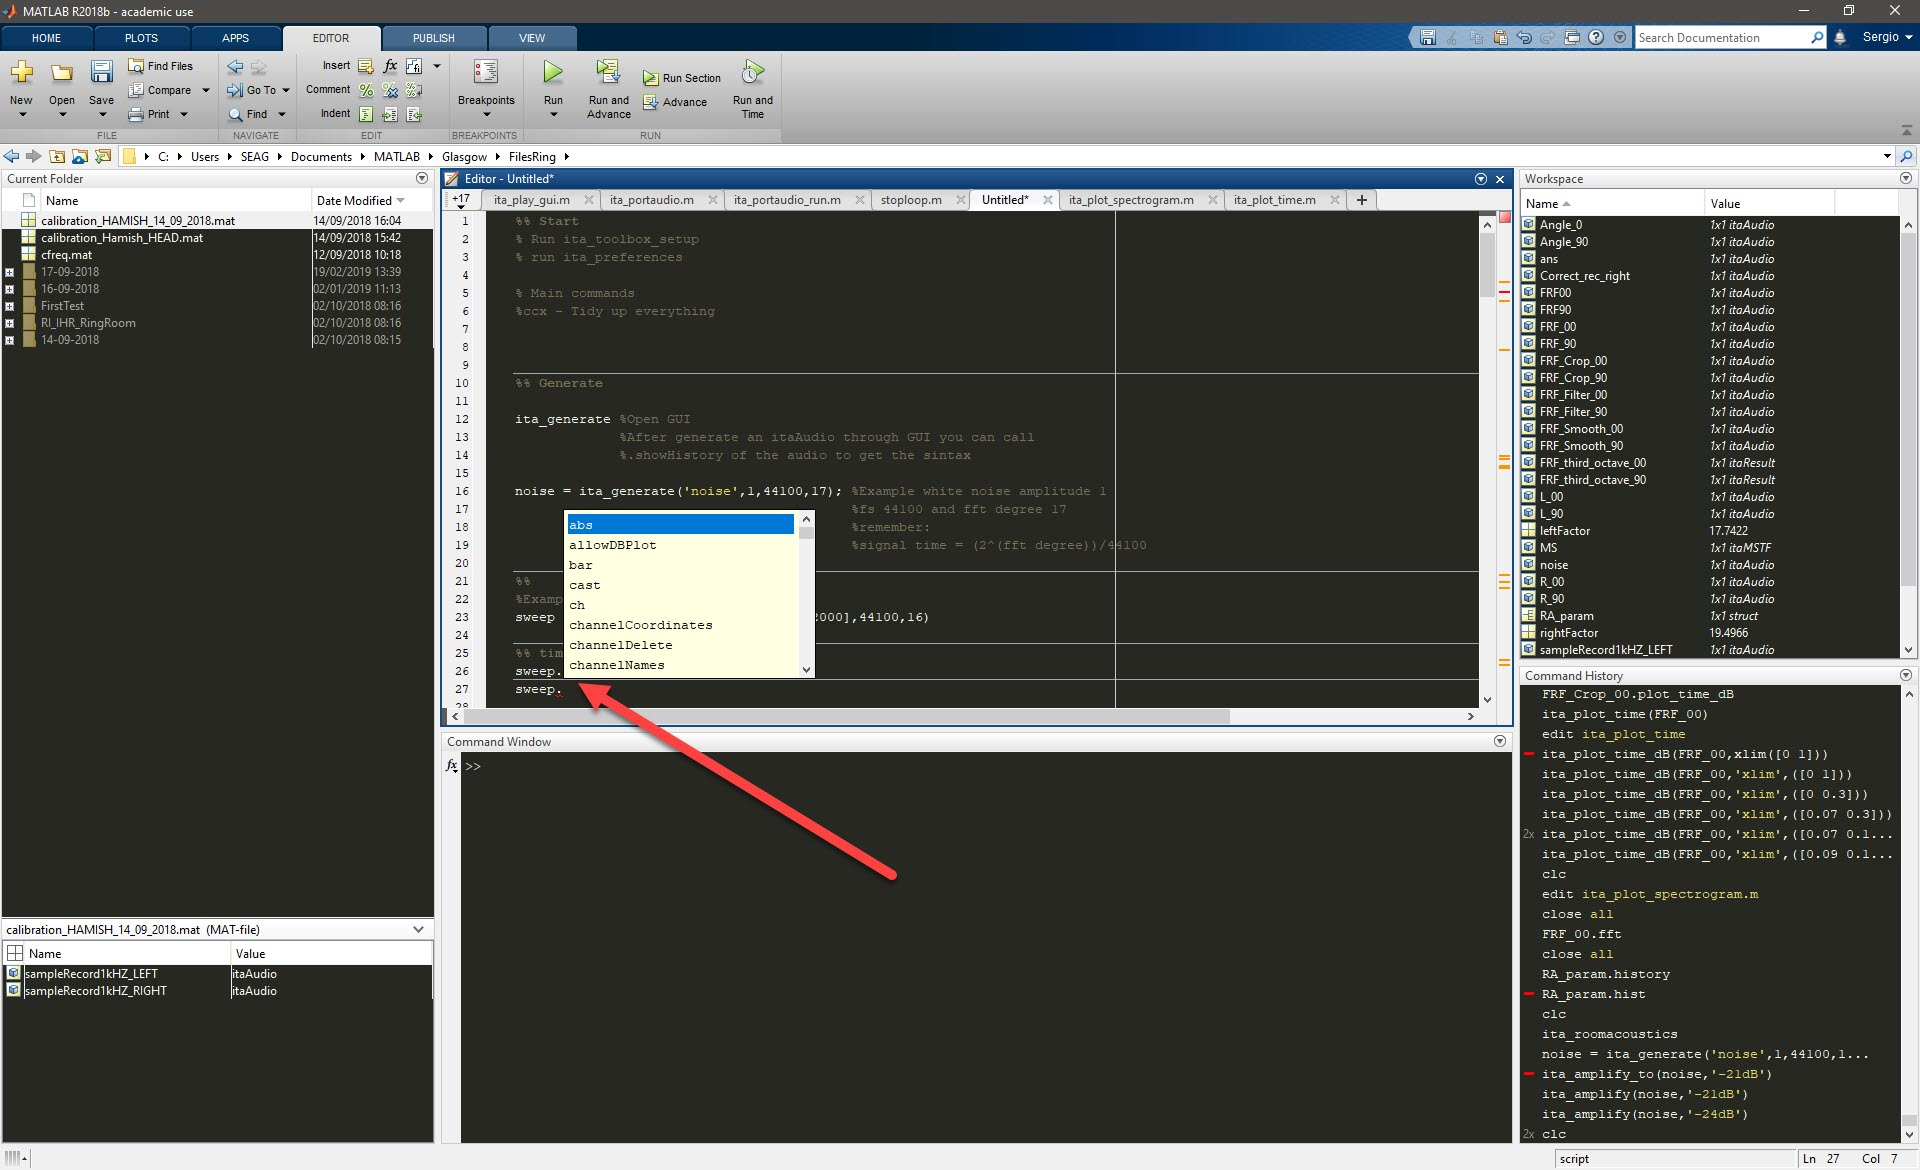
\includegraphics[width=.7\textwidth]{Figures/f7.jpg}
\end{figure}

\section*{Various Examples}
%%
\begin{matlabbox}
%% various examples

%load
load('Example_CHSI.mat')% Load old recorded sweeps
                                          % Two itaAudios
                                          % Each Angle has 2 channels
                                          % Left and Right ear from a HATS
                                          % Recorded in Glasgow last year
%% Sweep used to record (I remember the params)
signalReference = ita_generate('ccxsweep',[50 20000],44100,16); 
\end{matlabbox}

Let's plot all

\begin{matlabbox}
Angle_0.plot_all
\end{matlabbox}

\begin{figure}[H] \centering
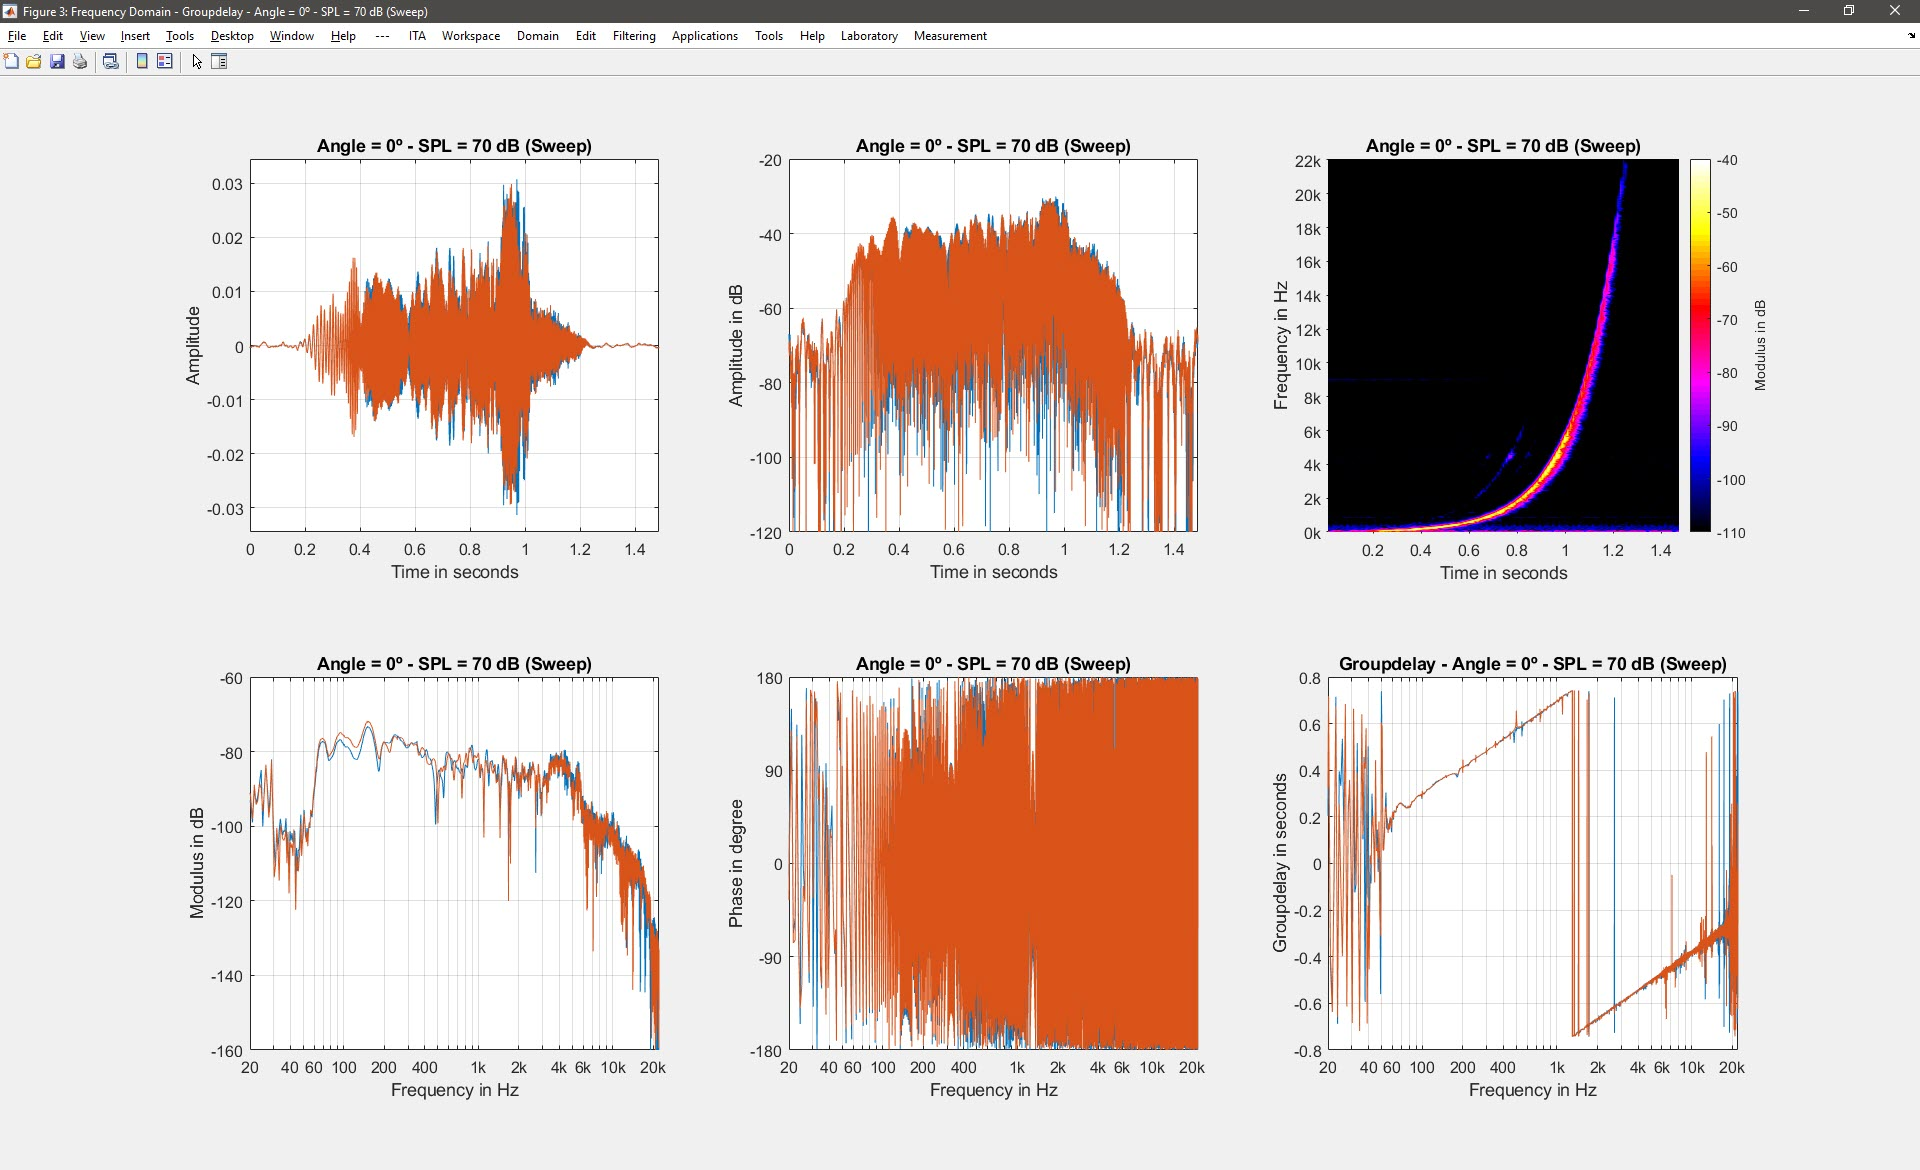
\includegraphics[width=.7\textwidth]{Figures/E1.jpg}
\end{figure}

I recommend you browse the menus\\
Domain, Edit, Filtering...
\begin{figure}[H] \centering
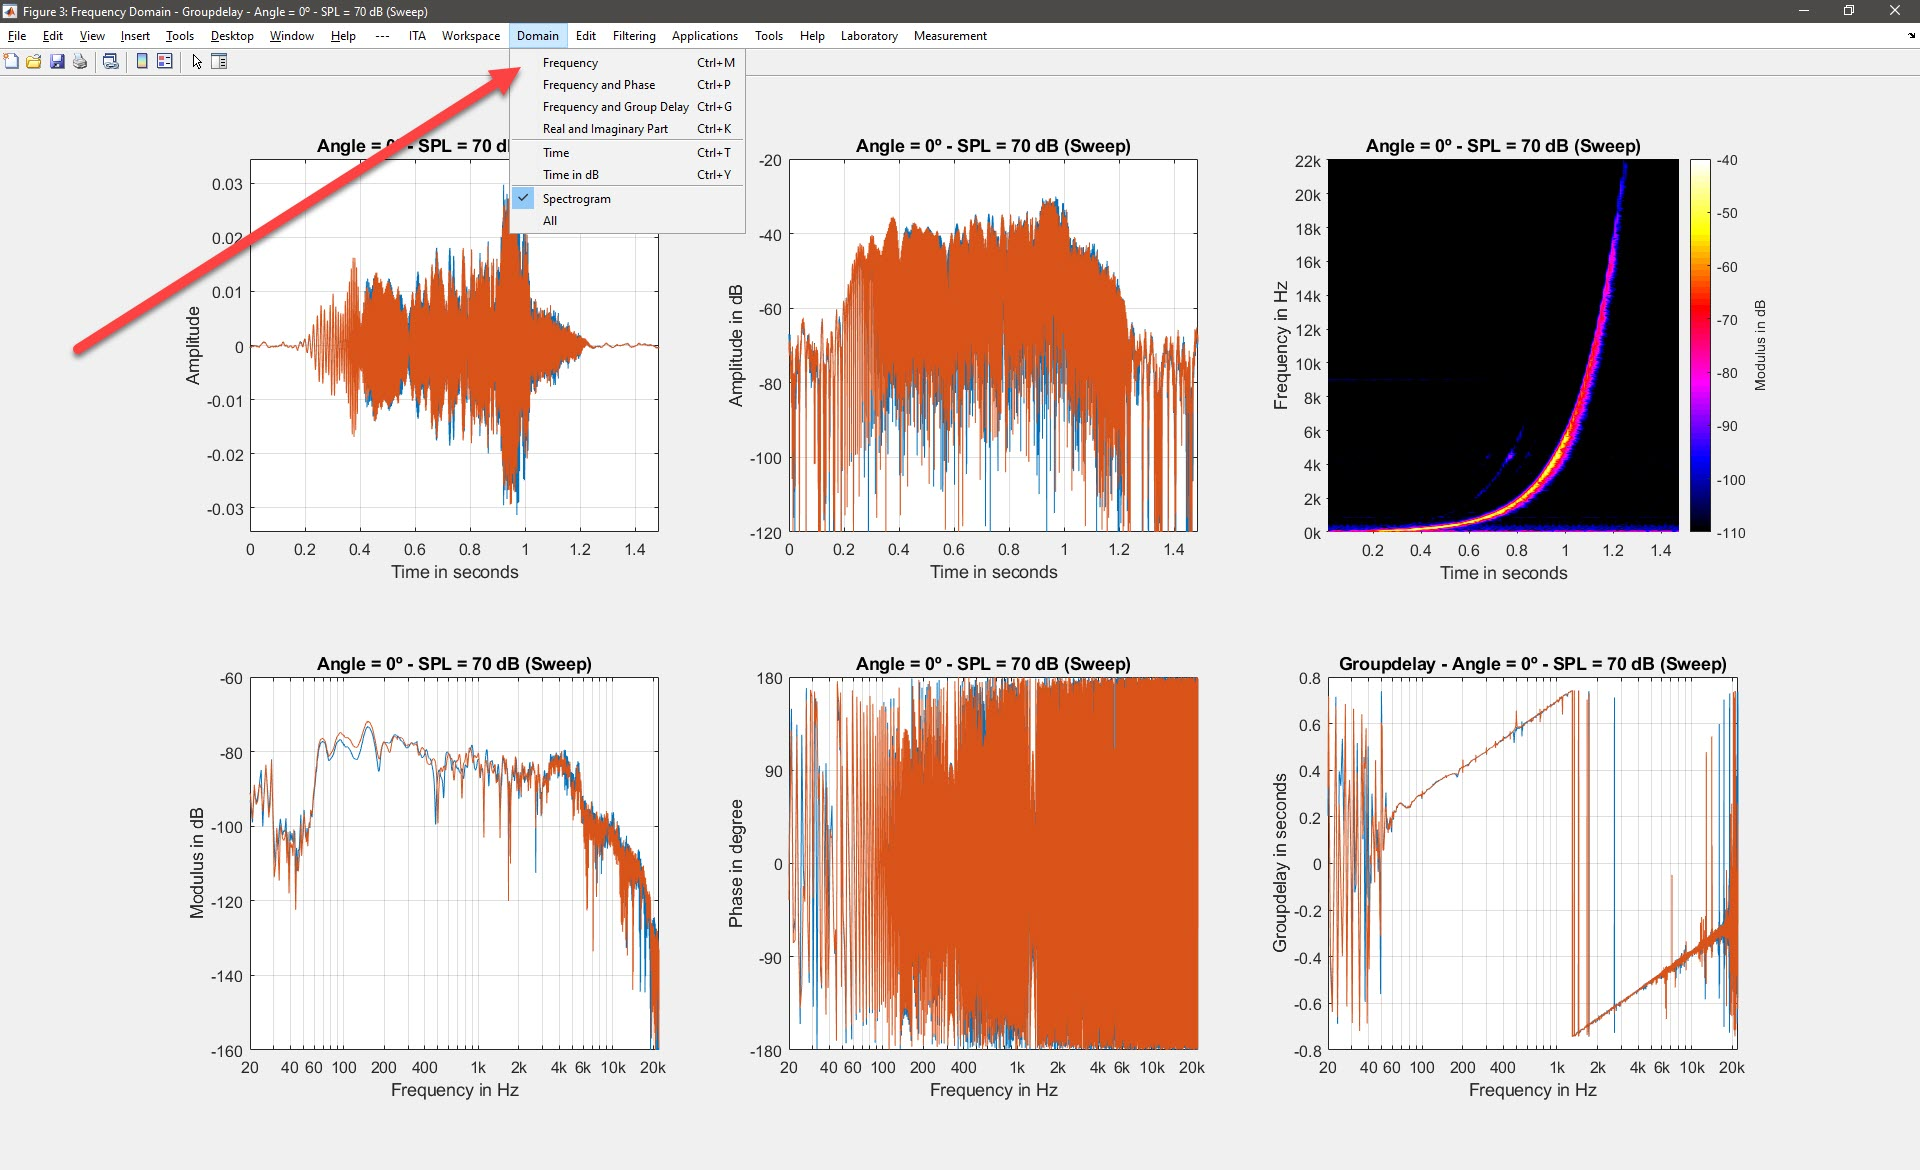
\includegraphics[width=.45\textwidth]{Figures/E2.jpg}
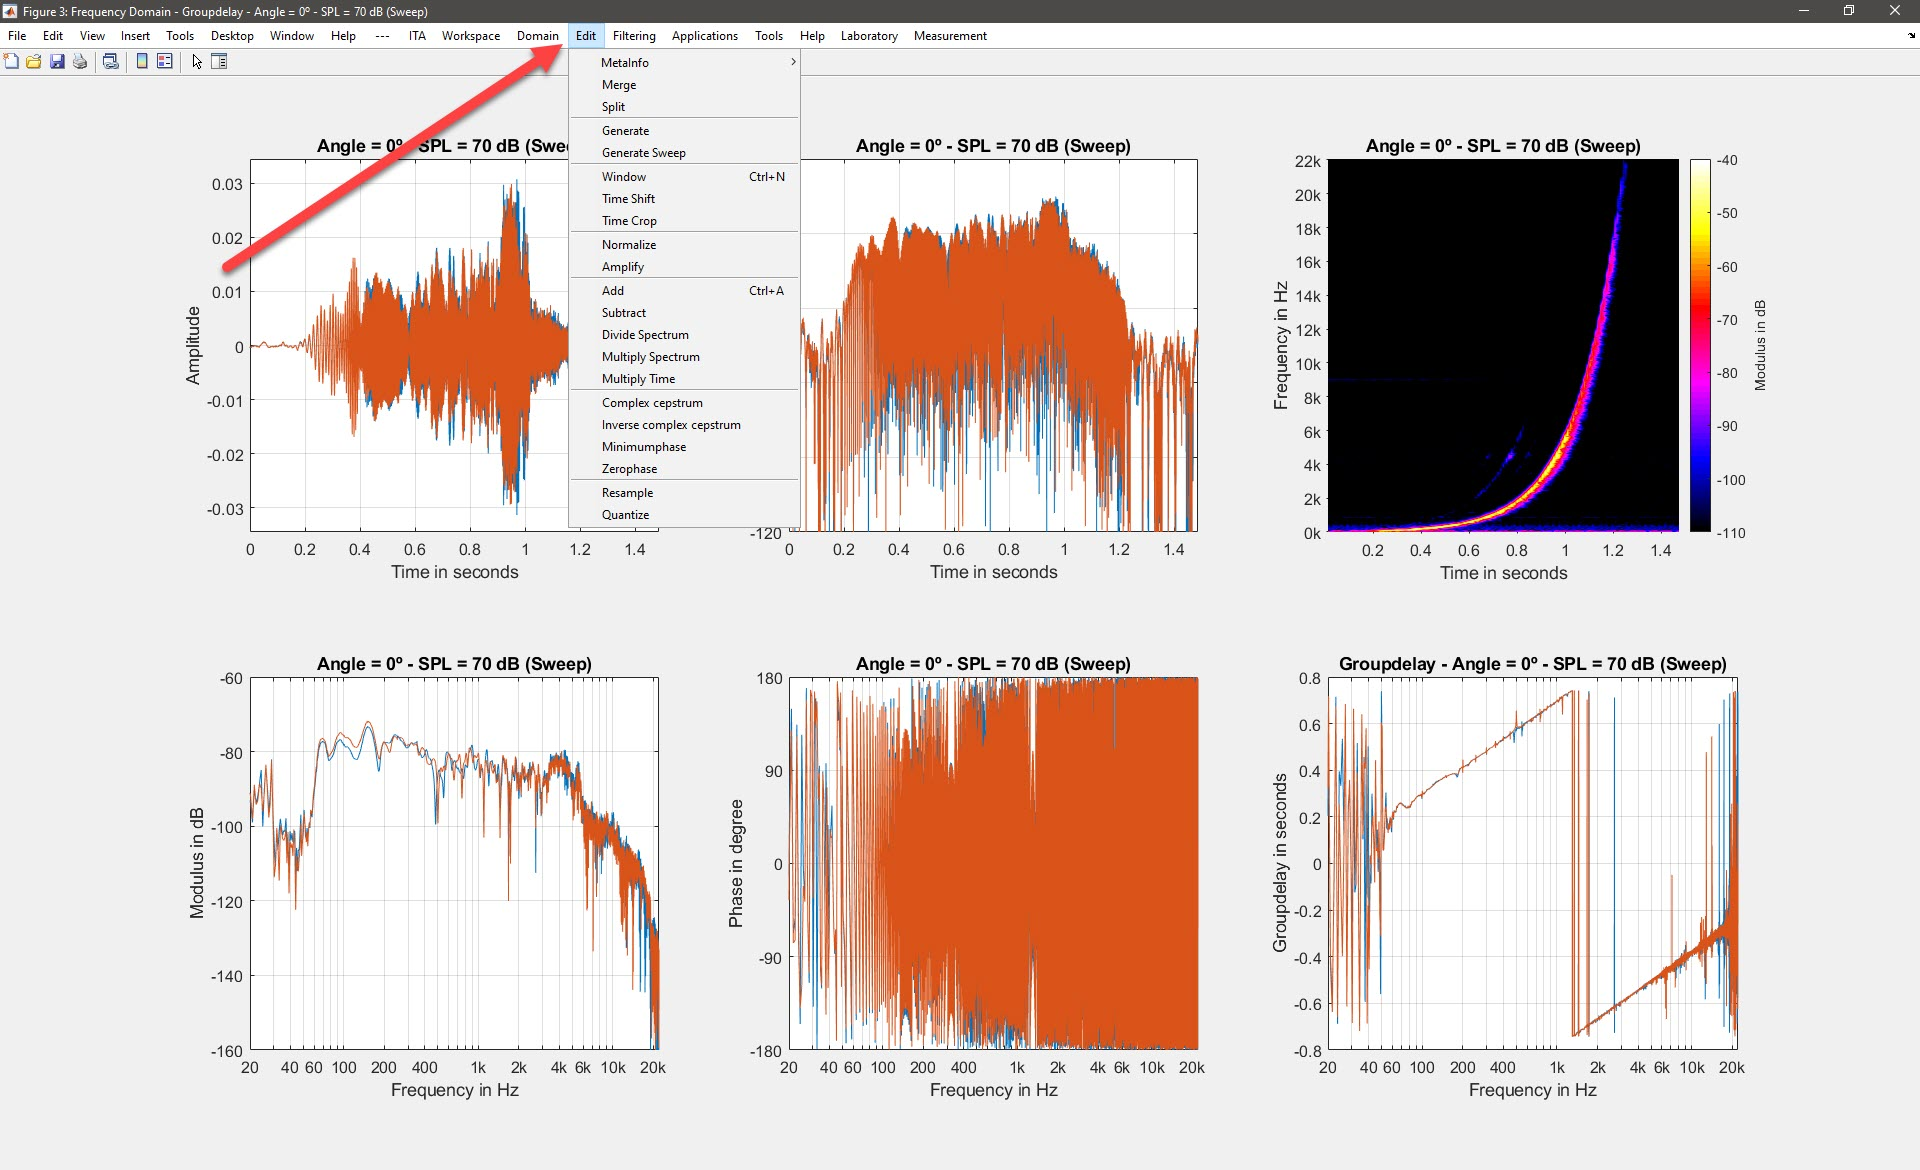
\includegraphics[width=.45\textwidth]{Figures/E3.jpg}
\end{figure}
\begin{figure}[H] \centering
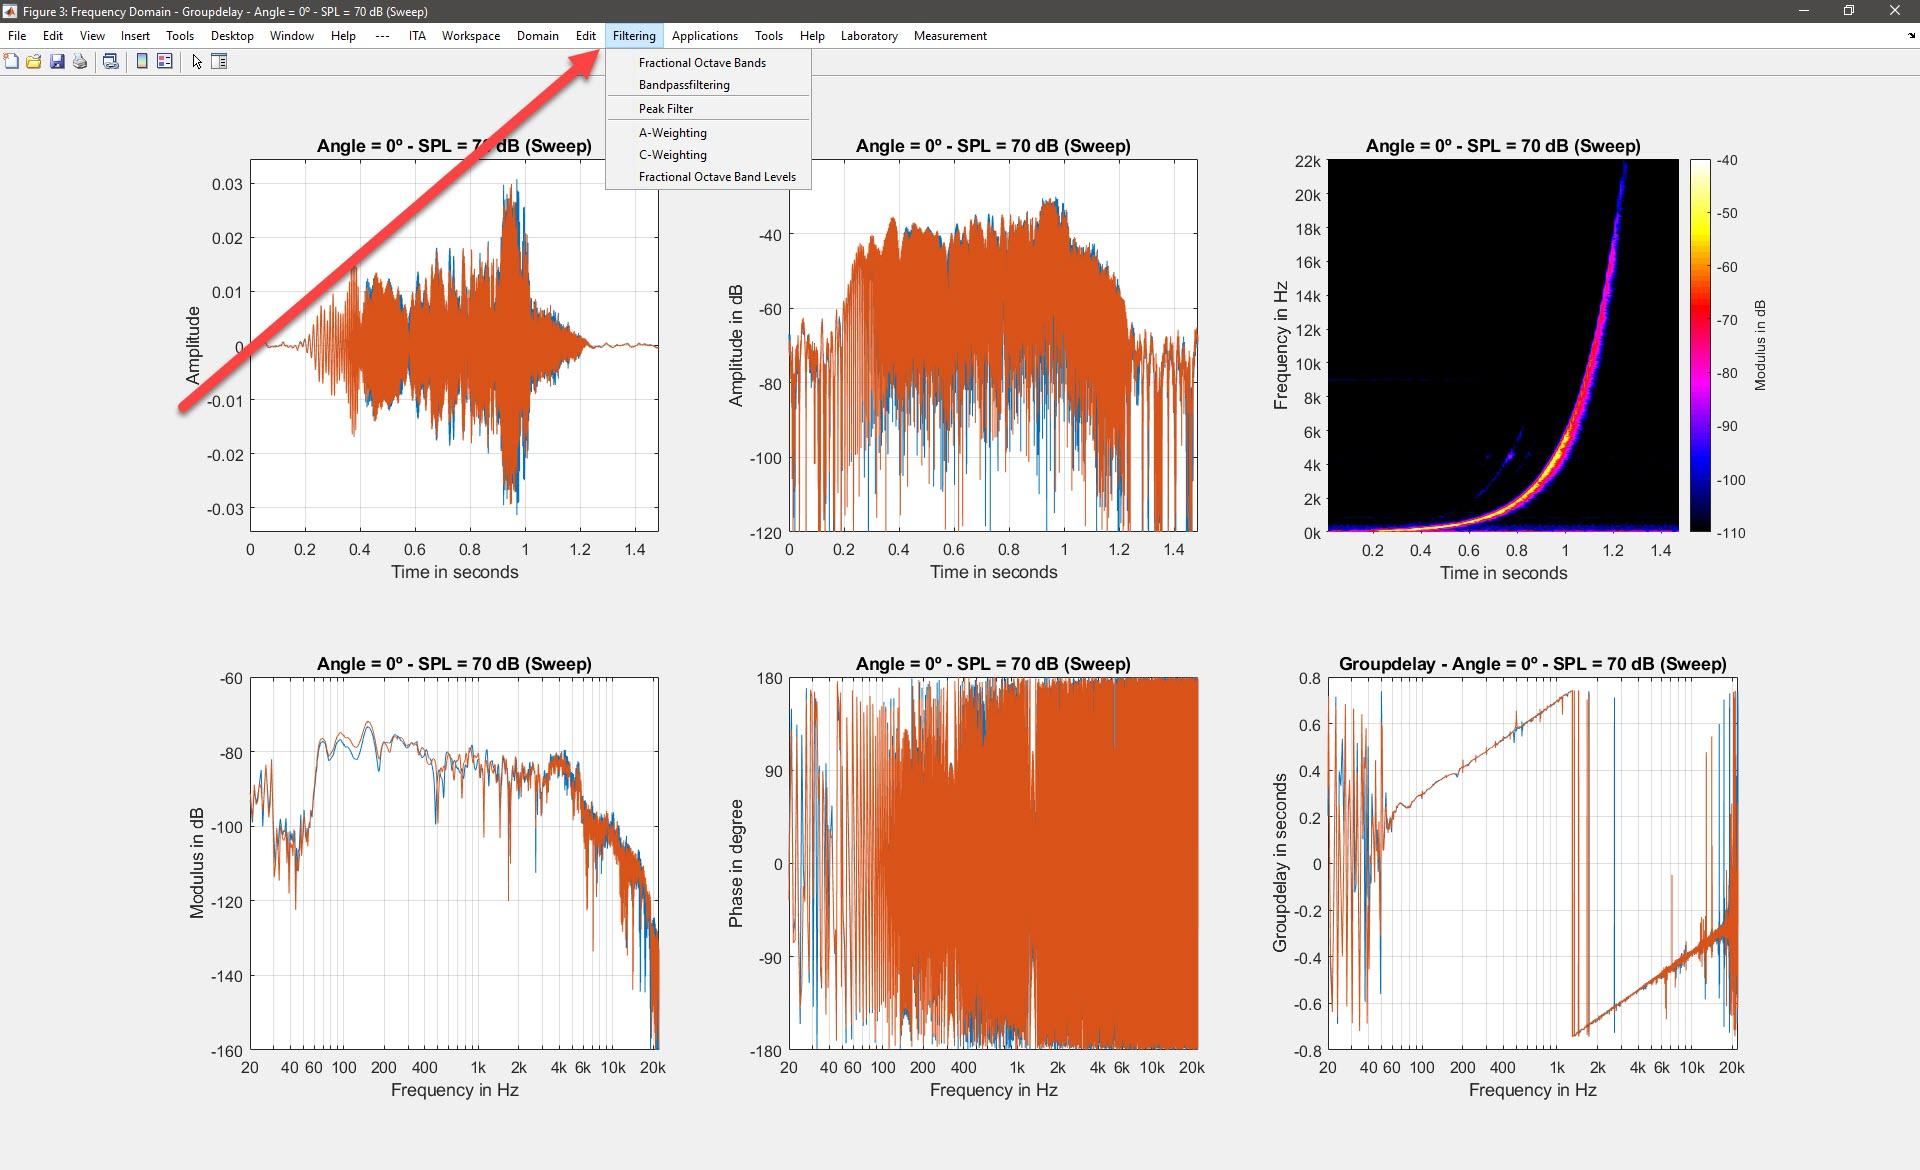
\includegraphics[width=.45\textwidth]{Figures/E4.jpg}
\end{figure}

\pagebreak
%%%%%%%%%%%%%%%%%%%%%%%%%%%%%%%%%%%%%%%%%%%%%%%%%%%%%%%%%%%%%%%
\begin{matlabbox}
%% Plot (time) both Recordings (4 channels)
ita_plot_time(merge(Angle_0,Angle_90))
\end{matlabbox}

\begin{figure}[H] \centering
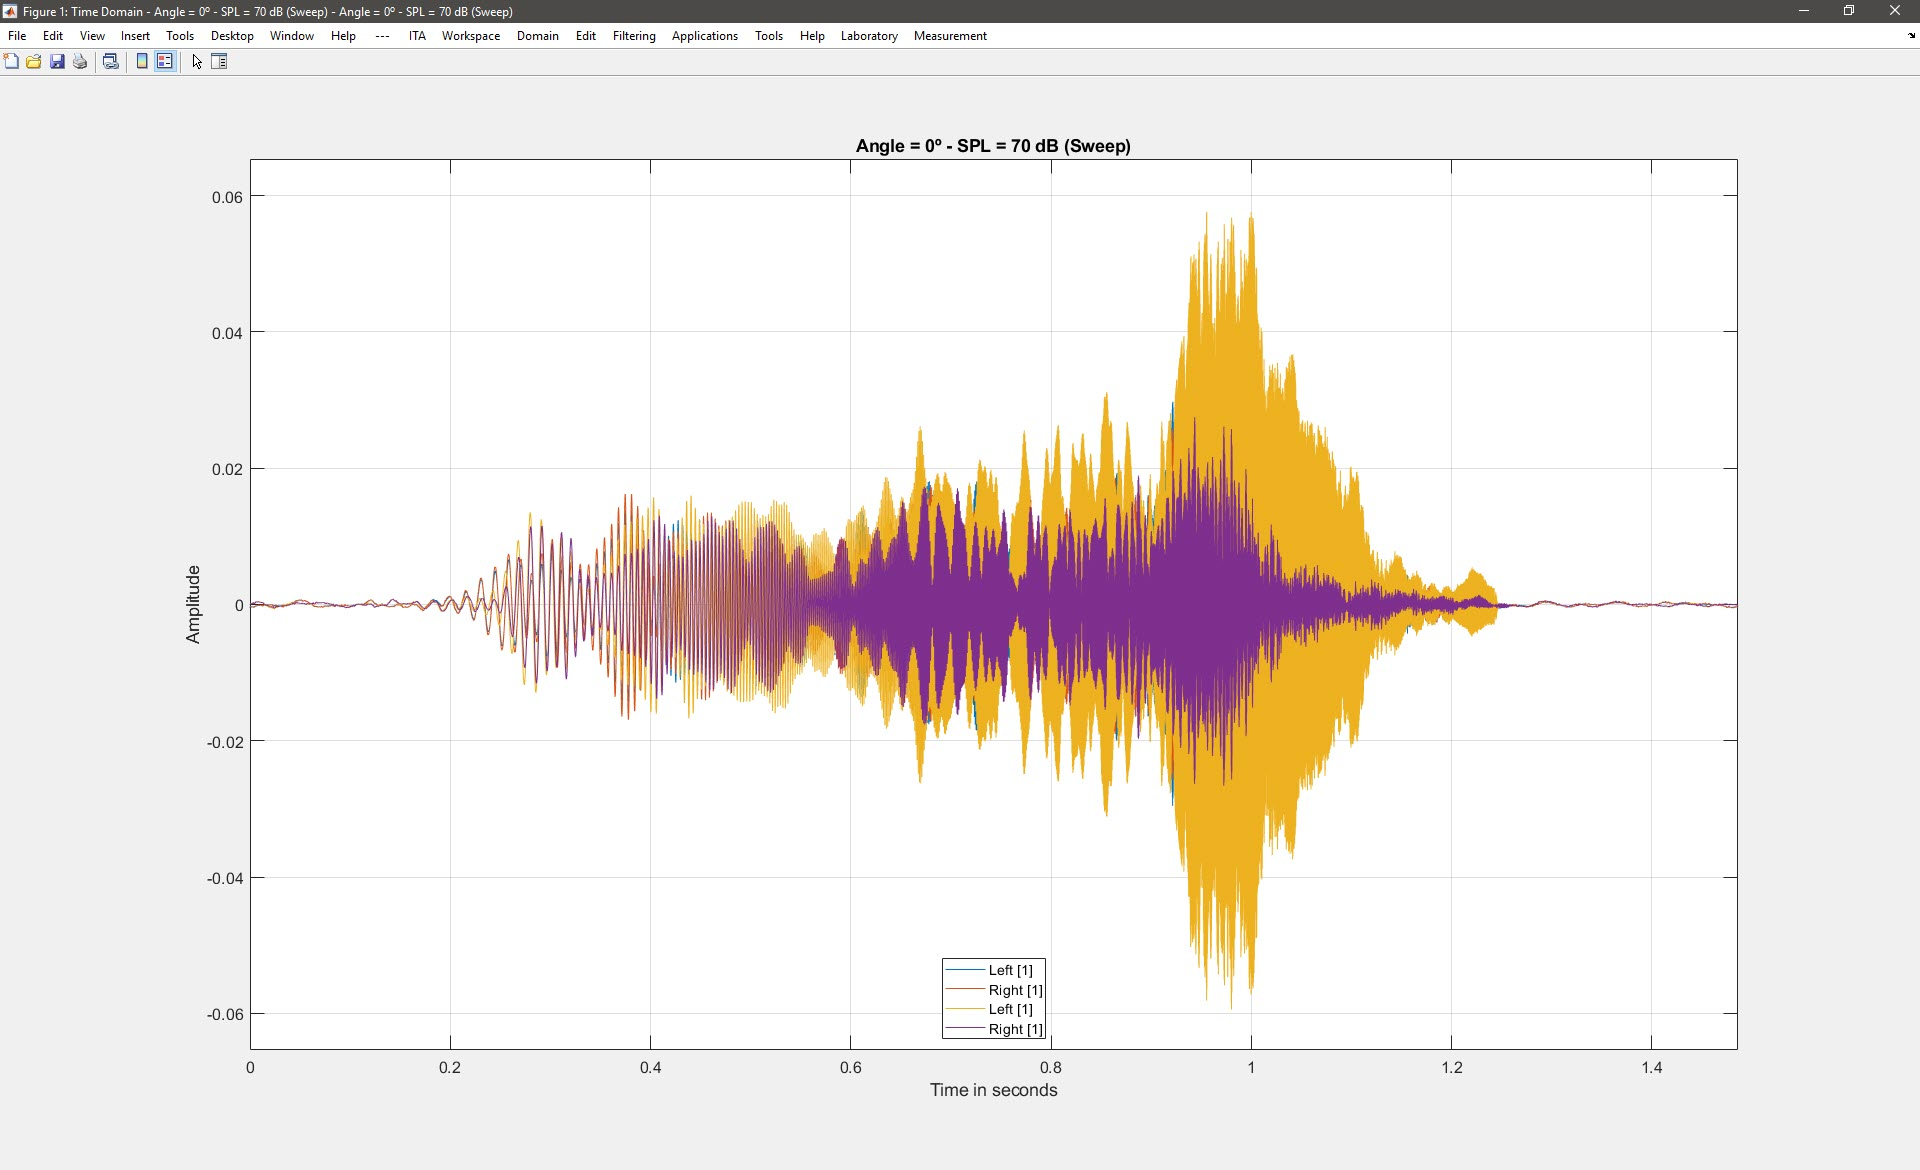
\includegraphics[width=.7\textwidth]{Figures/E5.jpg}
\end{figure}


%%%%%%%%%%%%%%%%%%%%%%%%%%%%%%%%%%%%%%%%%%%%%%%%%%%%%%%%%%%%%%%
\begin{matlabbox}
%% Calculate BRIR 
FRF_00 = ita_divide_spk(Angle_0,signalReference) % Use the freq division
%% Plot time
ita_plot_time(FRF_00)

\end{matlabbox}

\begin{figure}[H] \centering
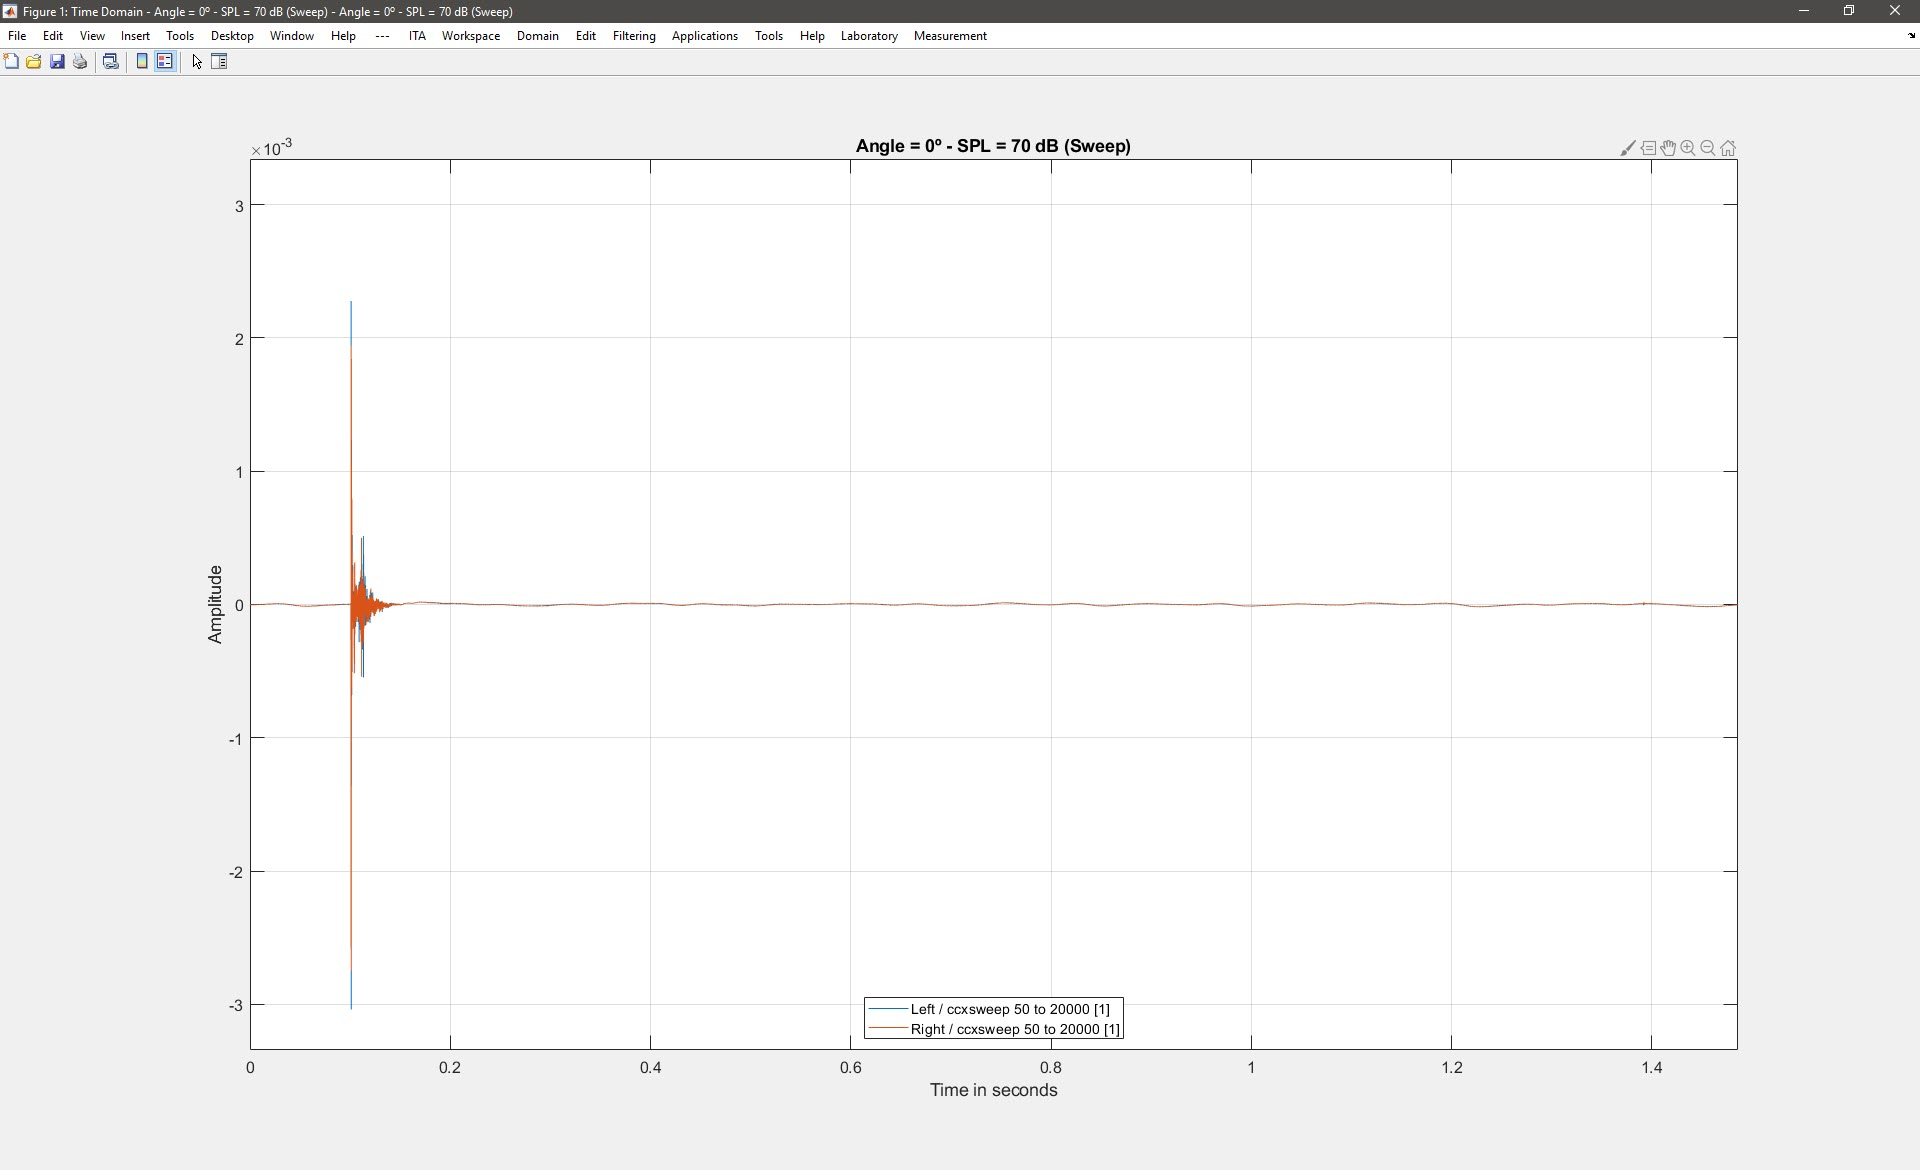
\includegraphics[width=.7\textwidth]{Figures/E6.jpg}
\end{figure}

%%%%%%%%%%%%%%%%%%%%%%%%%%%%%%%%%%%%%%%%%%%%%%%%%%%%%%%%%%%%%%%
\pagebreak
\begin{matlabbox}
%% Plot Freq
ita_plot_freq(FRF_00)
\end{matlabbox}
\begin{figure}[H] \centering
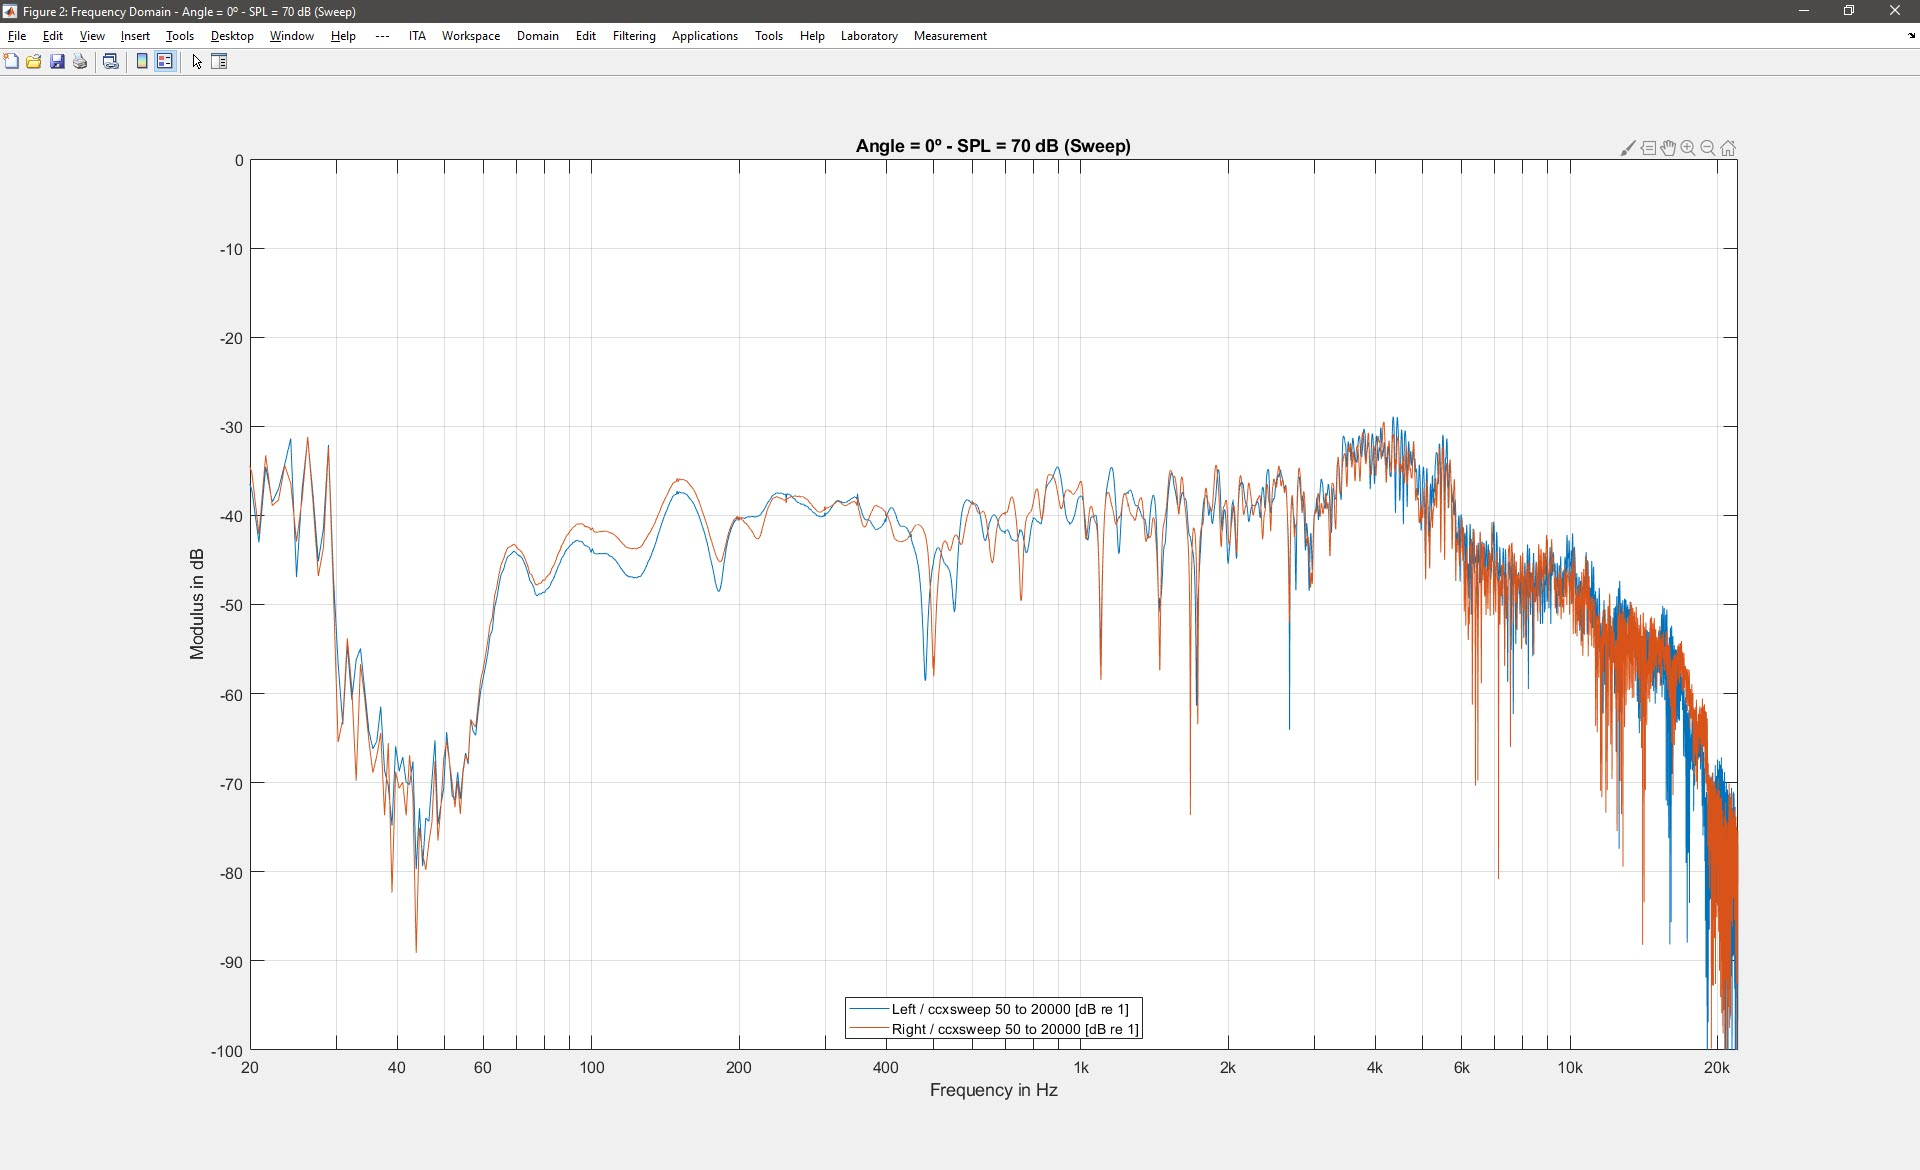
\includegraphics[width=.7\textwidth]{Figures/E7.jpg}
\end{figure}

%%%%%%%%%%%%%%%%%%%%%%%%%%%%%%%%%%%%%%%%%%%%%%%%%%%%%%%%%%%%%%%
\begin{matlabbox}
%% Plot time in dB
ita_plot_time_dB(FRF_00)
\end{matlabbox}
\begin{figure}[H] \centering
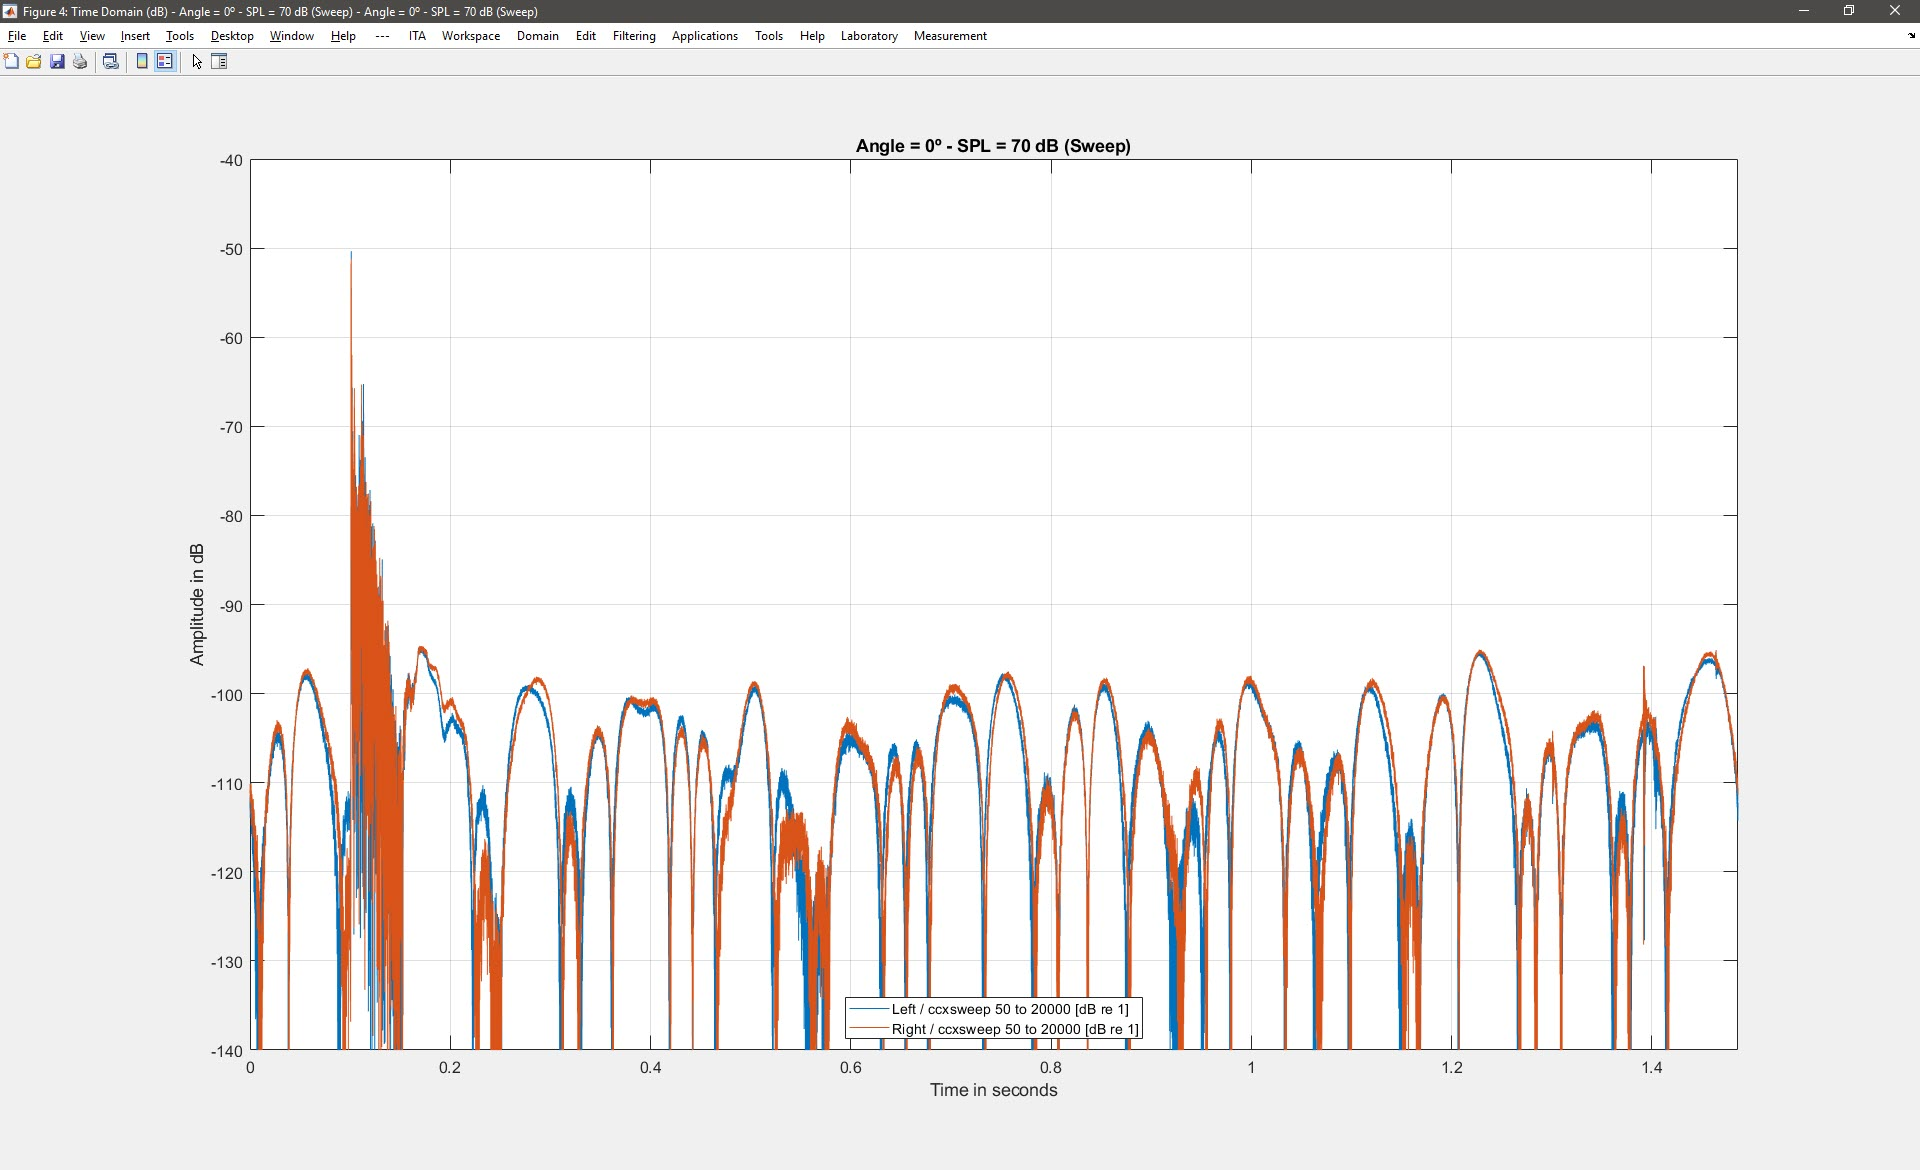
\includegraphics[width=.7\textwidth]{Figures/E8.jpg}
\end{figure}
\pagebreak
%%%%%%%%%%%%%%%%%%%%%%%%%%%%%%%%%%%%%%%%%%%%%%%%%%%%%%%%%%%%%%%
\begin{matlabbox}
%% Looking closer to see DS, ER and LR
ita_plot_time_dB(FRF_00,'xlim',([0.09 0.15]))

\end{matlabbox}
\begin{figure}[H] \centering
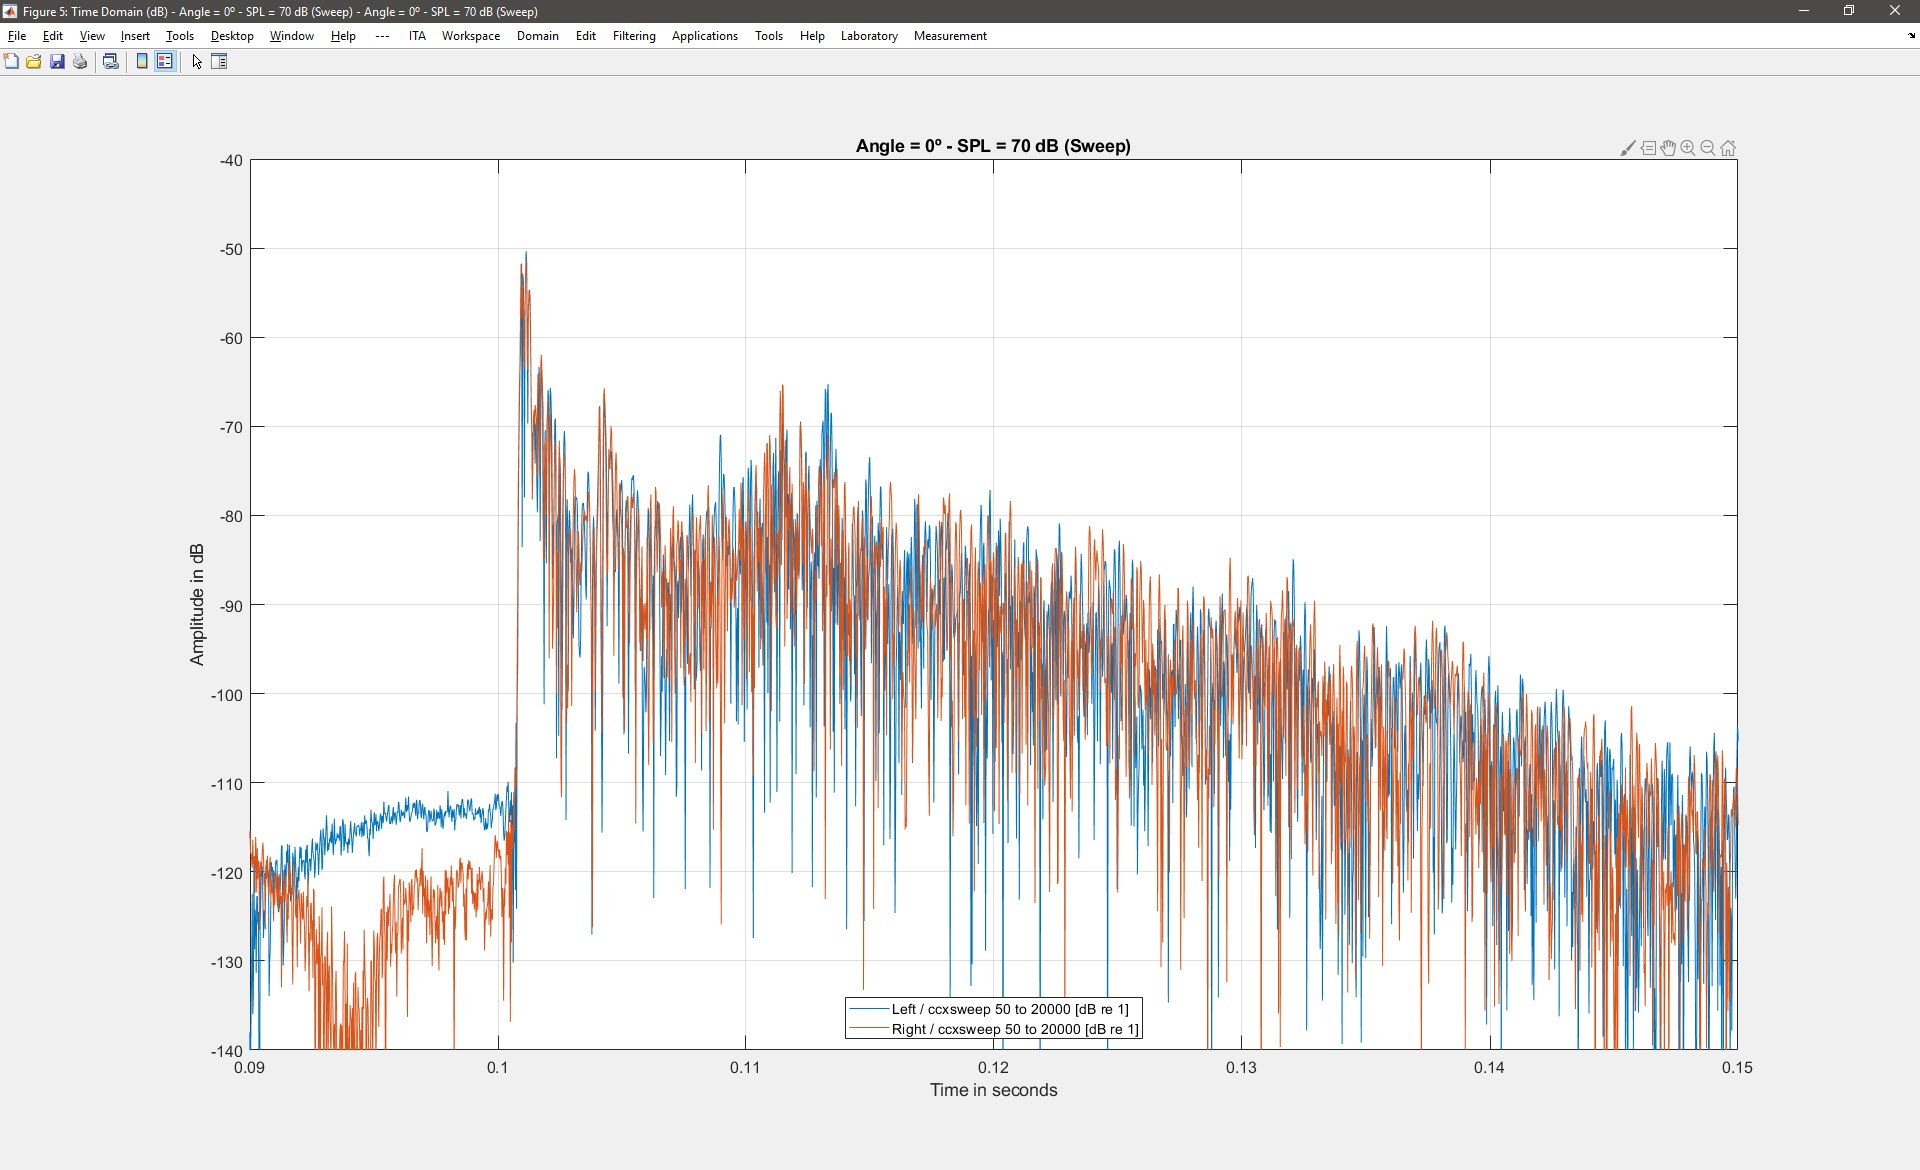
\includegraphics[width=.7\textwidth]{Figures/E9.jpg}
\end{figure}
%%%%%%%%%%%%%%%%%%%%%%%%%%%%%%%%%%%%%%%%%%%%%%%%%%%%%%%%%%%%%%%
\begin{matlabbox}
%% Spectrogram with Artemis colors
ita_plot_spectrogram(FRF_00)
\end{matlabbox}
\begin{figure}[H] \centering
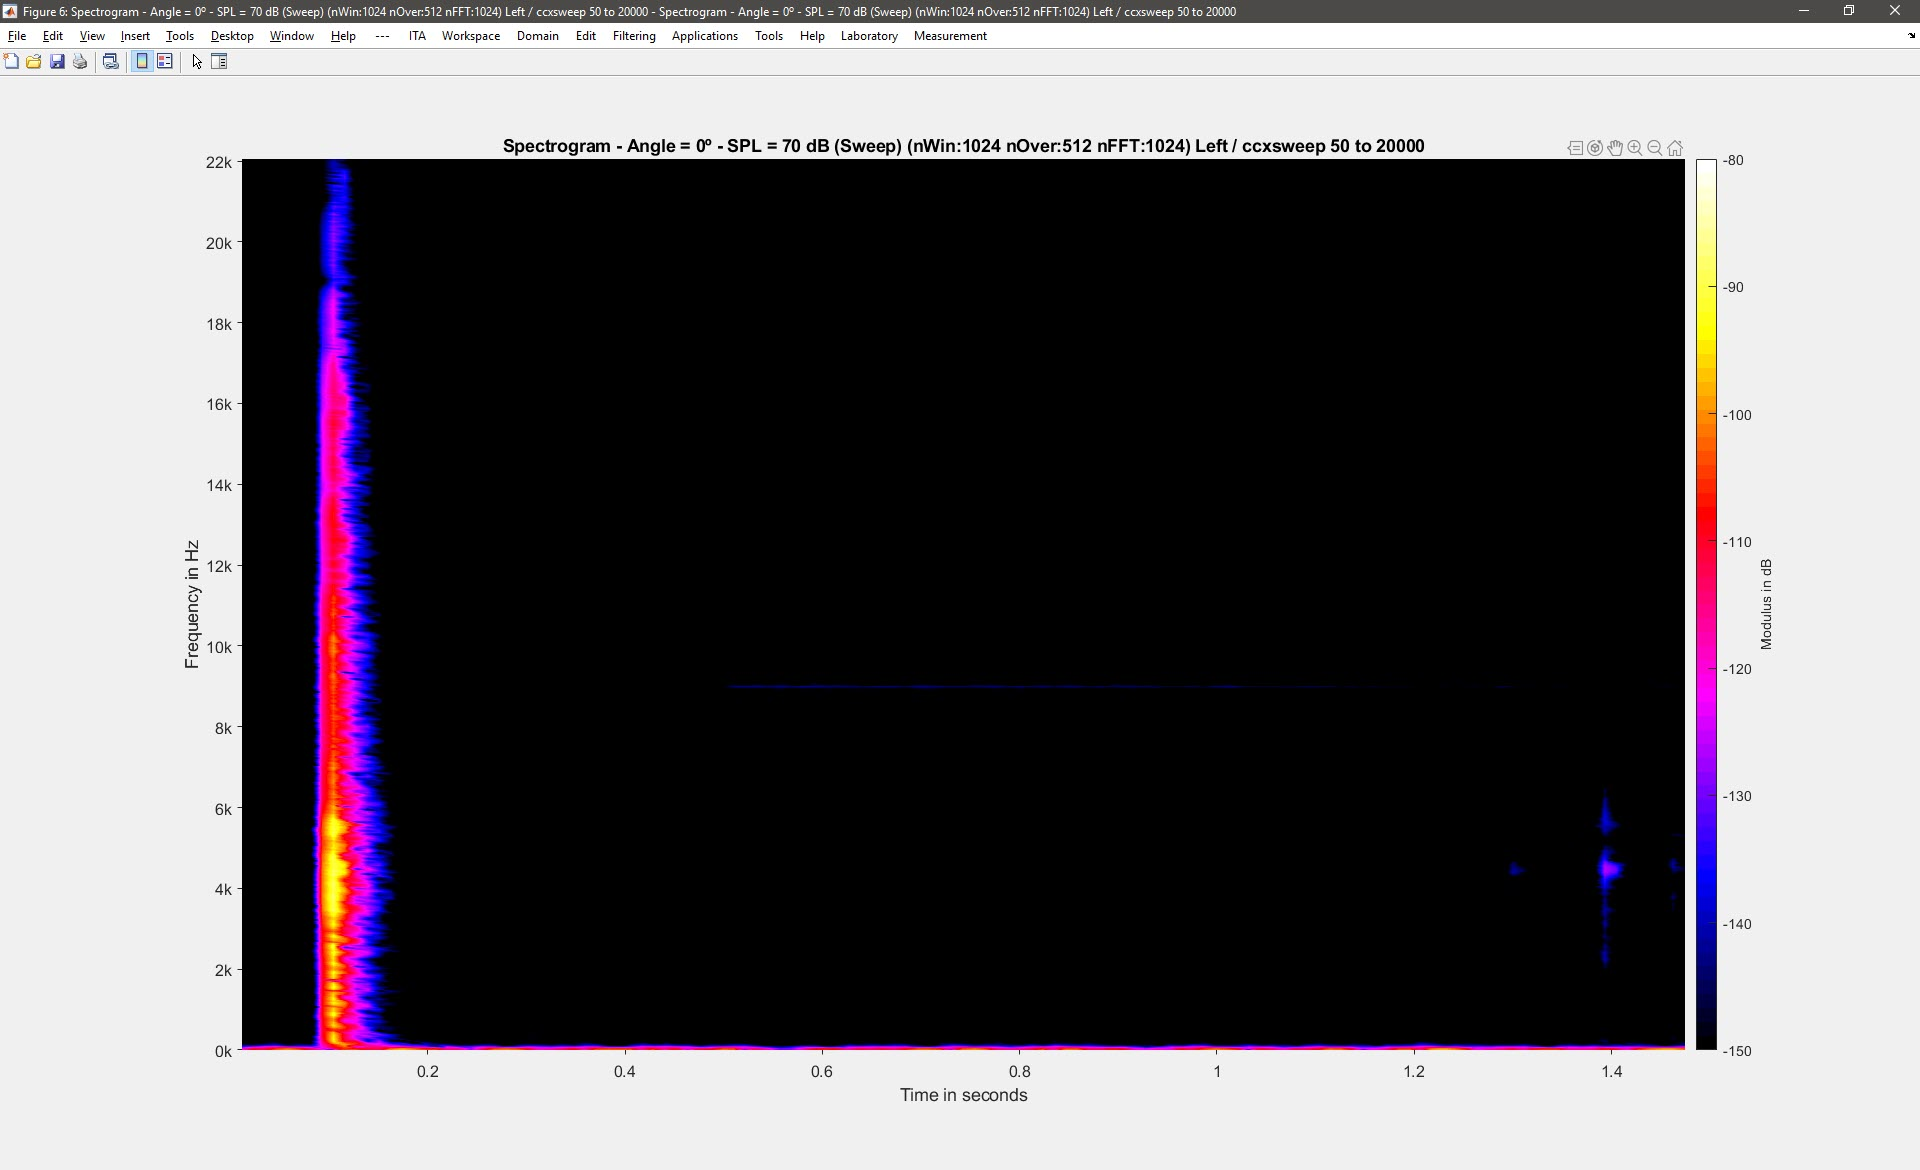
\includegraphics[width=.7\textwidth]{Figures/E10.jpg}
\end{figure}

%%%%%%%%%%%%%%%%%%%%%%%%%%%%%%%%%%%%%%%%%%%%%%%%%%%%%%%%%%%%%%%
\pagebreak
%%%%%%%%%%%%%%%%%%%%%%%%%%%%%%%%%%%%%%%%%%%%%%%%%%%%%%%%%%%%%%%
\begin{matlabbox}
%% Change some options
ita_plot_spectrogram(FRF_00,'ylog',(true),'nodb',true)
ylabel('Frequency in kHz')
\end{matlabbox}
\begin{figure}[H] \centering
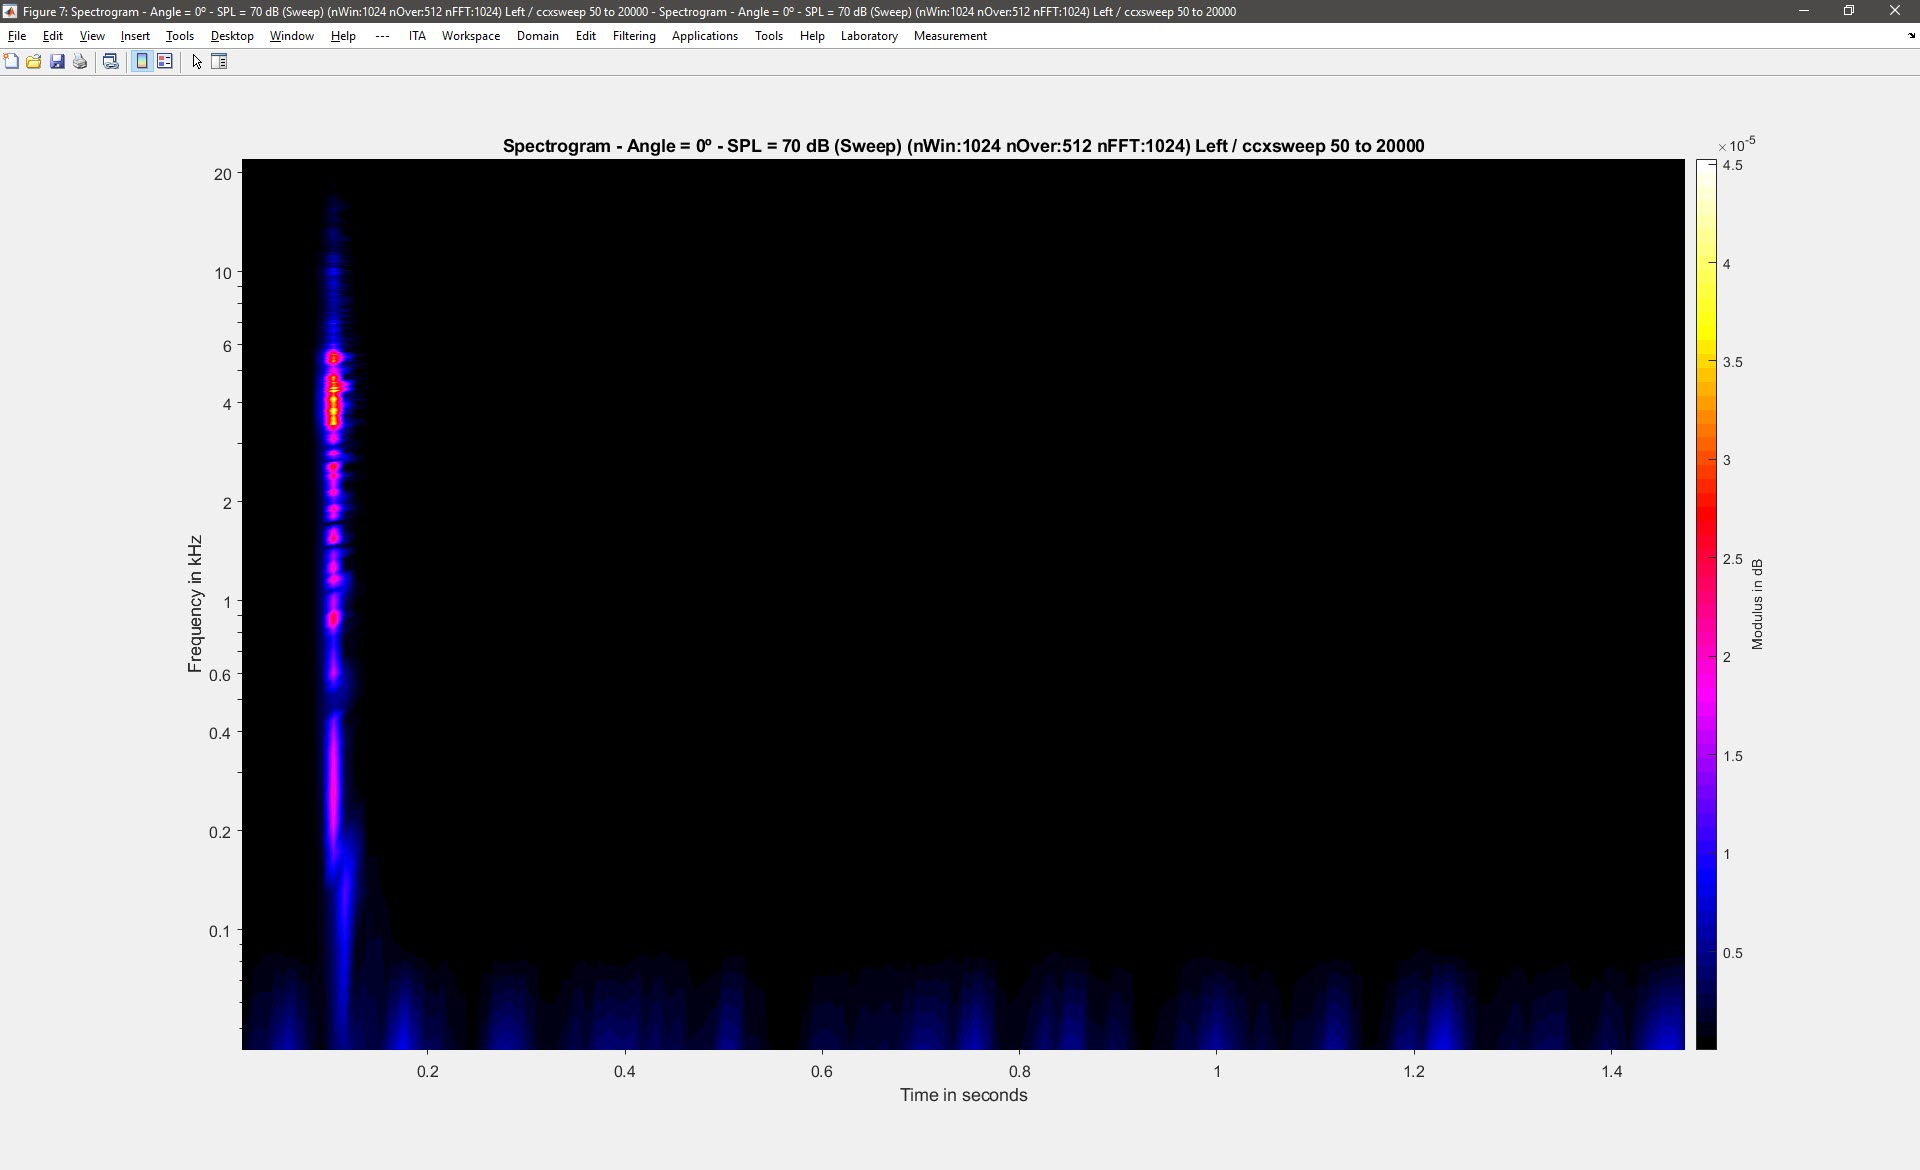
\includegraphics[width=.7\textwidth]{Figures/E11.jpg}
\end{figure}


%%%%%%%%%%%%%%%%%%%%%%%%%%%%%%%%%%%%%%%%%%%%%%%%%%%%%%%%%%%%%%%
\begin{matlabbox}
%%
FRF_90 = ita_divide_spk(Angle_90,signalReference); %
%% Crop at specific time
FRF_Crop_00 = ita_time_crop(FRF_00,[0 0.2],'time'); %Crop
FRF_Crop_90 = ita_time_crop(FRF_90,[0 0.2],'time'); %Crop 

%% Plot Cropped 
FRF_Crop_00.plot_time

\end{matlabbox}
\begin{figure}[H] \centering
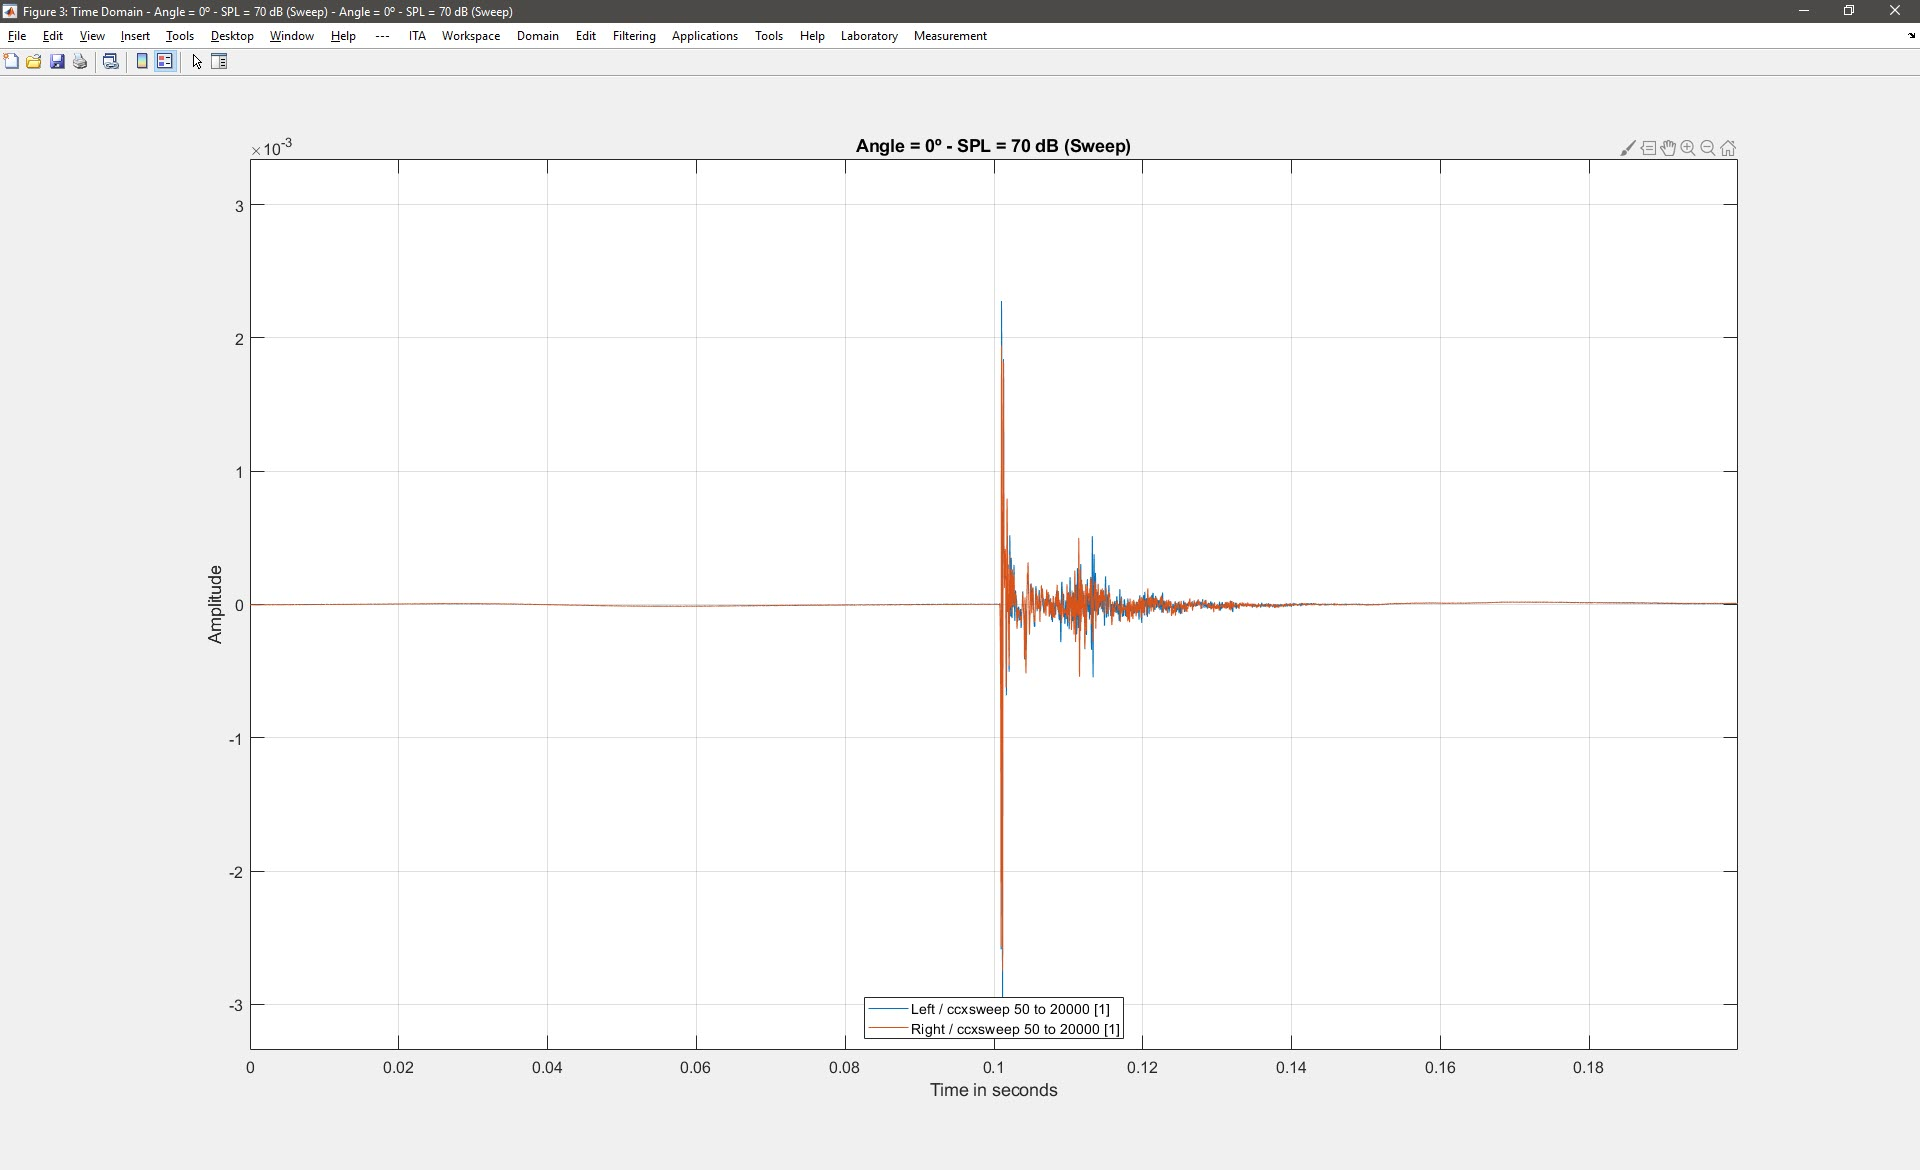
\includegraphics[width=.7\textwidth]{Figures/E12.jpg}
\end{figure}
%%%%%%%%%%%%%%%%%%%%%%%%%%%%%%%%%%%%%%%%%%%%%%%%%%%%%%%%%%%%%%%
\pagebreak
%%%%%%%%%%%%%%%%%%%%%%%%%%%%%%%%%%%%%%%%%%%%%%%%%%%%%%%%%%%%%%%
\begin{matlabbox}
%% Smooth 
FRF_Smooth_00 = ita_smooth_frequency(FRF_Crop_00); %Smooth
FRF_Smooth_90 = ita_smooth_frequency(FRF_Crop_90); %Smooth

%% Plot smooth vs raw in freq
ita_plot_freq(merge(FRF_Crop_00,FRF_Smooth_00))
\end{matlabbox}
\begin{figure}[H] \centering
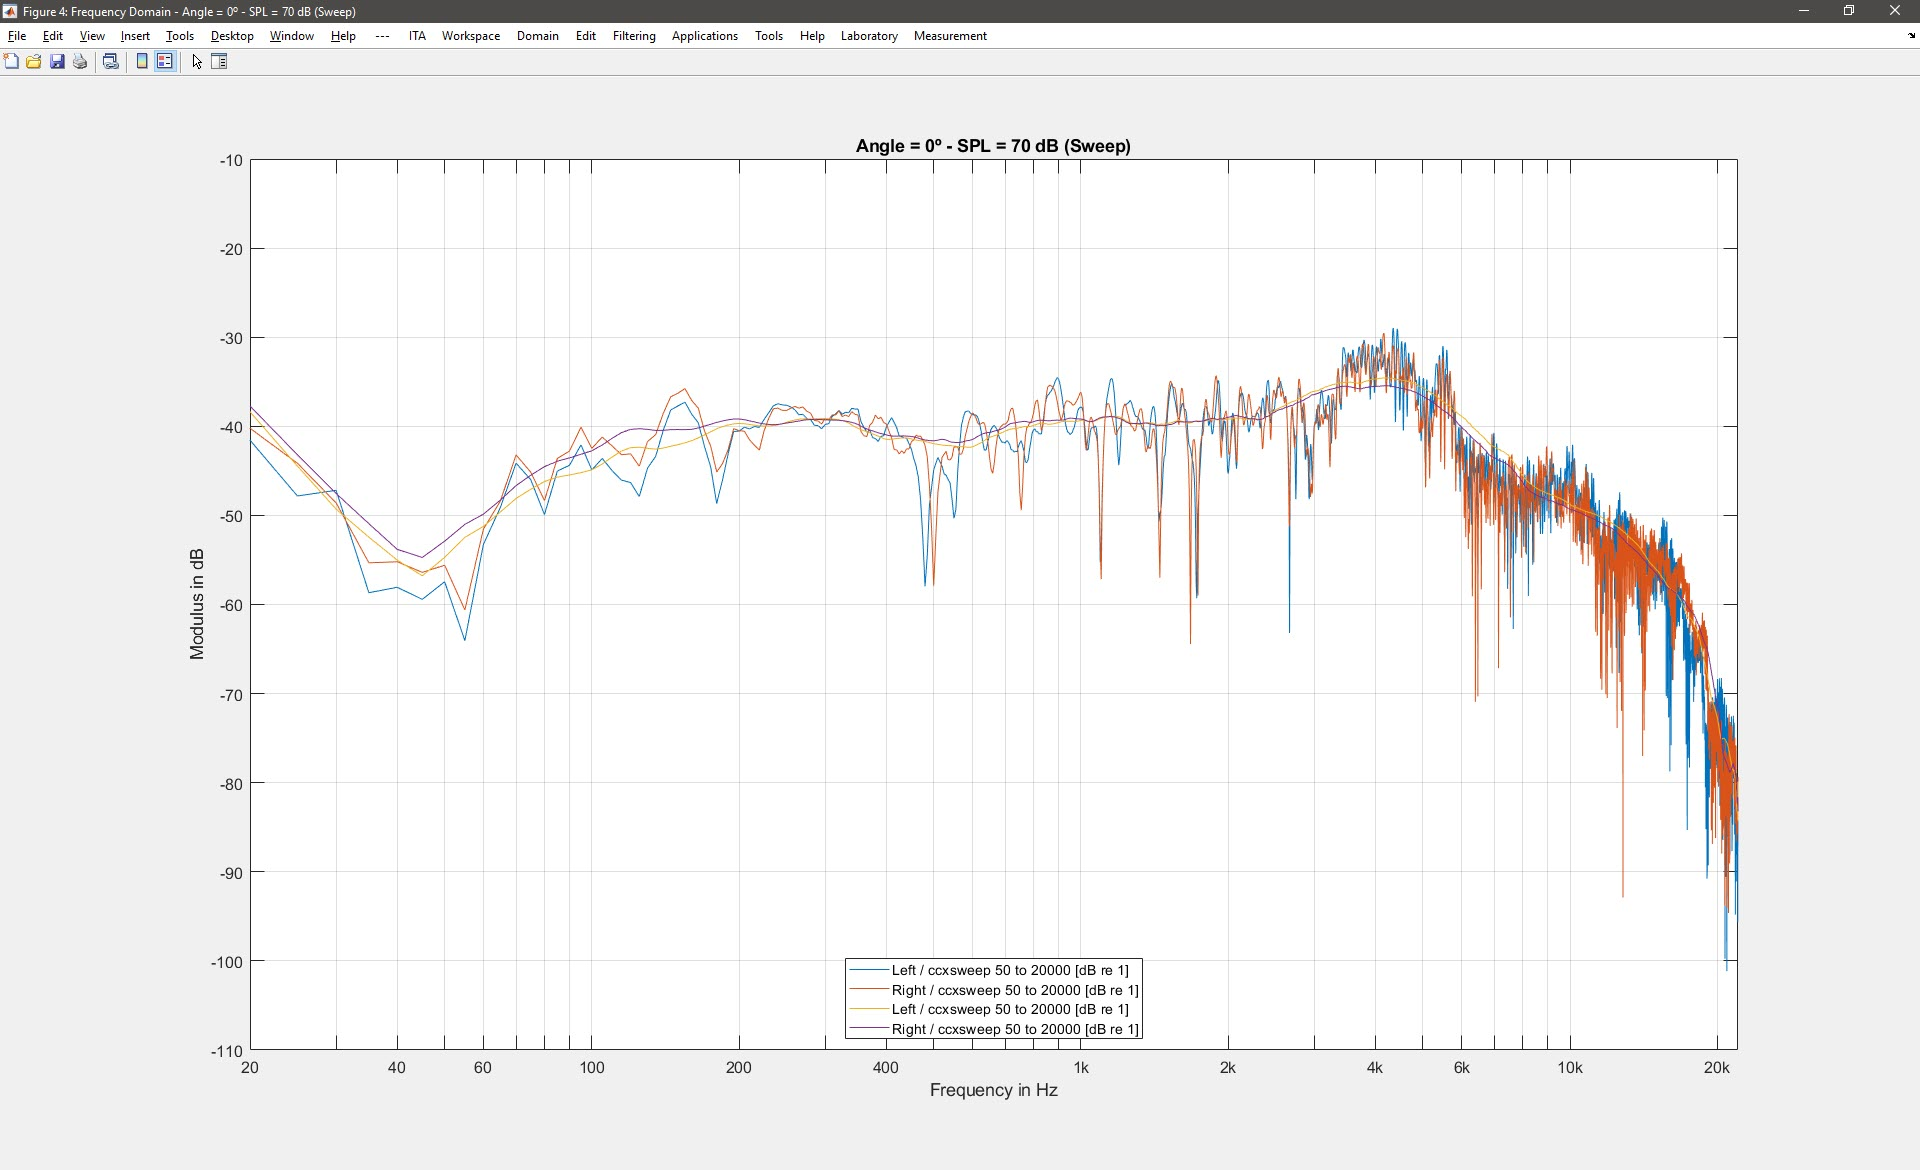
\includegraphics[width=.7\textwidth]{Figures/E13.jpg}
\end{figure}
%%%%%%%%%%%%%%%%%%%%%%%%%%%%%%%%%%%%%%%%%%%%%%%%%%%%%%%%%%%%%%%


%%%%%%%%%%%%%%%%%%%%%%%%%%%%%%%%%%%%%%%%%%%%%%%%%%%%%%%%%%%%%%%
\begin{matlabbox}
%% Split vectors
[L_00, R_00] = ita_split(FRF_Smooth_00,2,1); %Split 00
[L_90, R_90] = ita_split(FRF_Smooth_00,2,1); %Split 90

%% Load recordings sine from pistonphone 10 Pa
load('calibration_HAMISH_14_09_2018.mat') 

ita_plot_freq(sampleRecord1kHZ_RIGHT) %% LPlot freq *right side
\end{matlabbox}
\begin{figure}[H] \centering
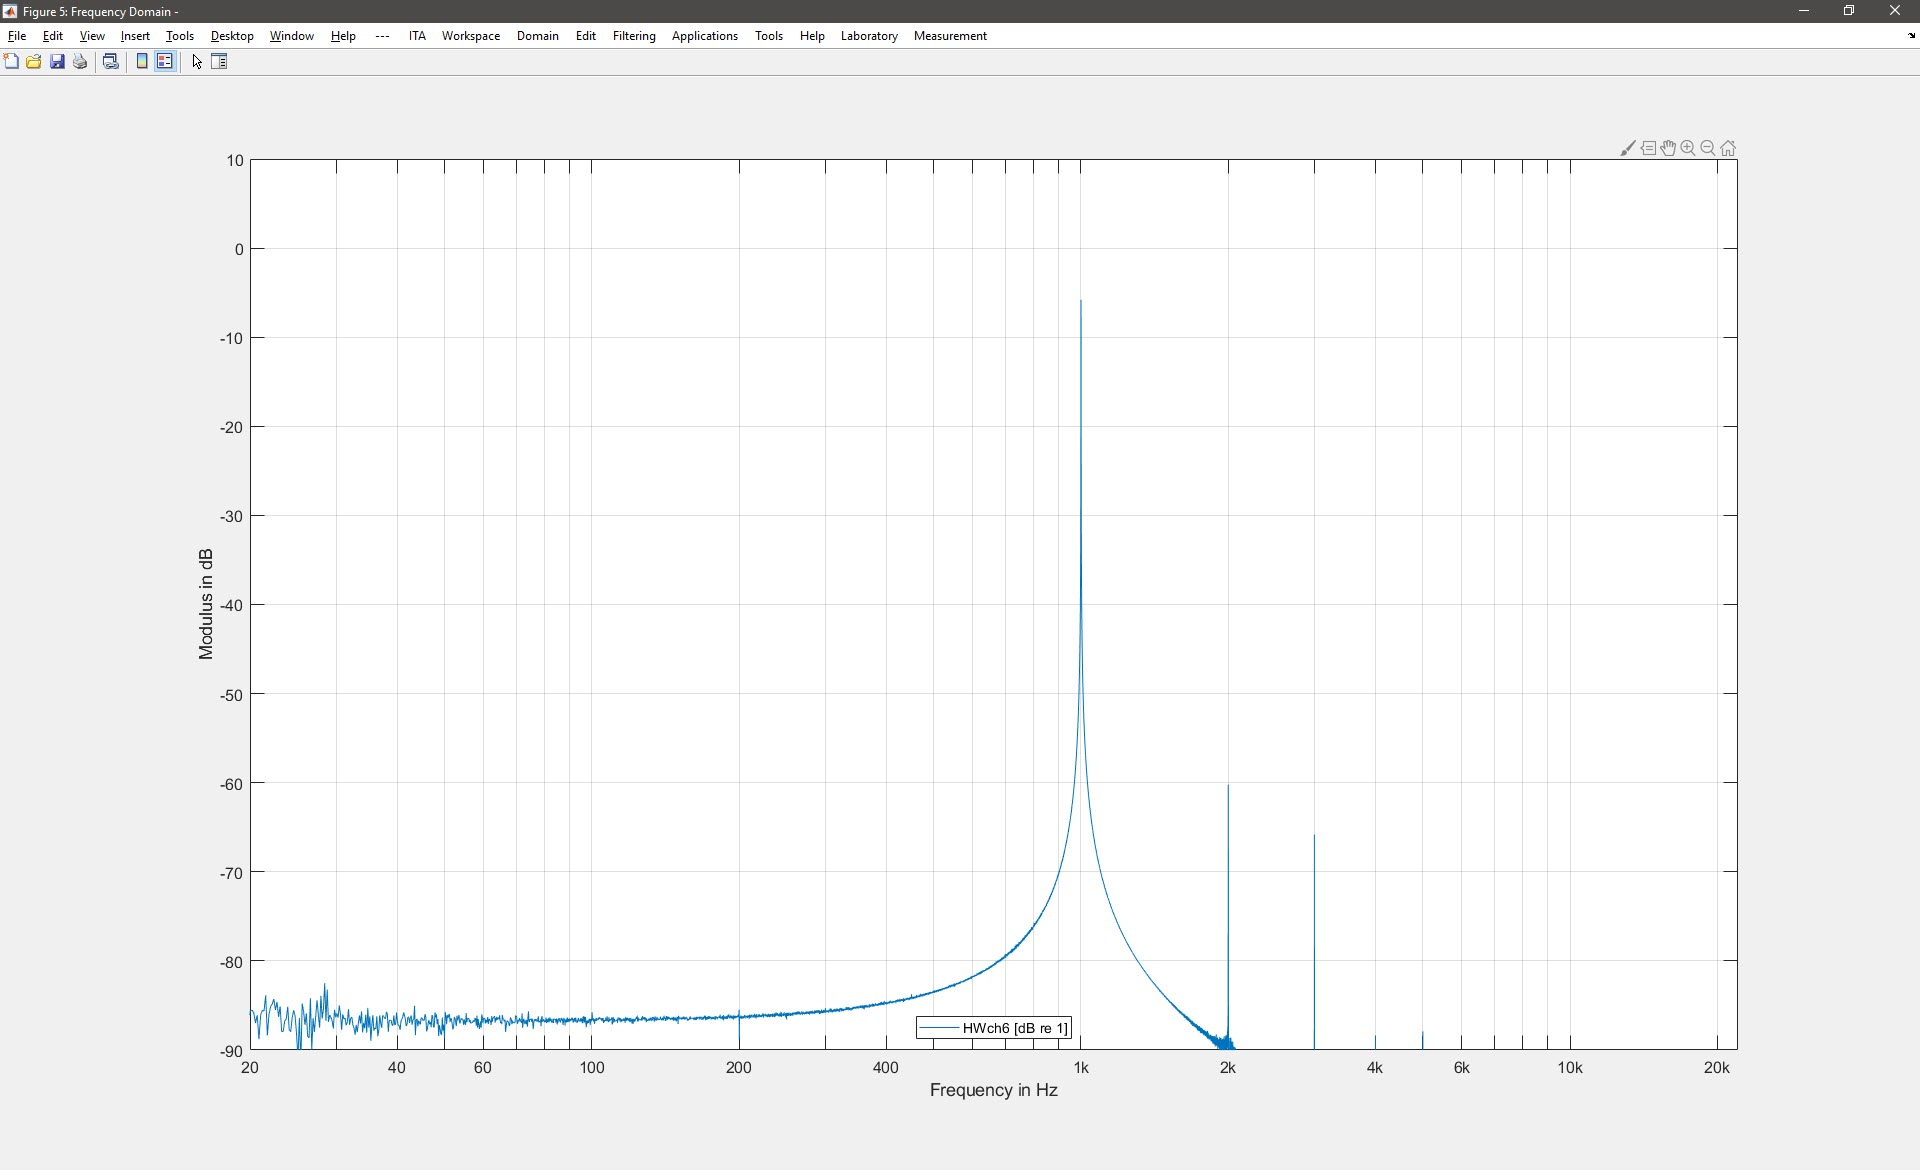
\includegraphics[width=.7\textwidth]{Figures/E14.jpg}
\end{figure}
%%%%%%%%%%%%%%%%%%%%%%%%%%%%%%%%%%%%%%%%%%%%%%%%%%%%%%%%%%%%%%%

\pagebreak
%%%%%%%%%%%%%%%%%%%%%%%%%%%%%%%%%%%%%%%%%%%%%%%%%%%%%%%%%%%%%%%
\begin{matlabbox}
%% Plot freq *right side changing the reference to 20 micro Pascal directly
ita_plot_freq(sampleRecord1kHZ_RIGHT/2e-5)

\end{matlabbox}
\begin{figure}[H] \centering
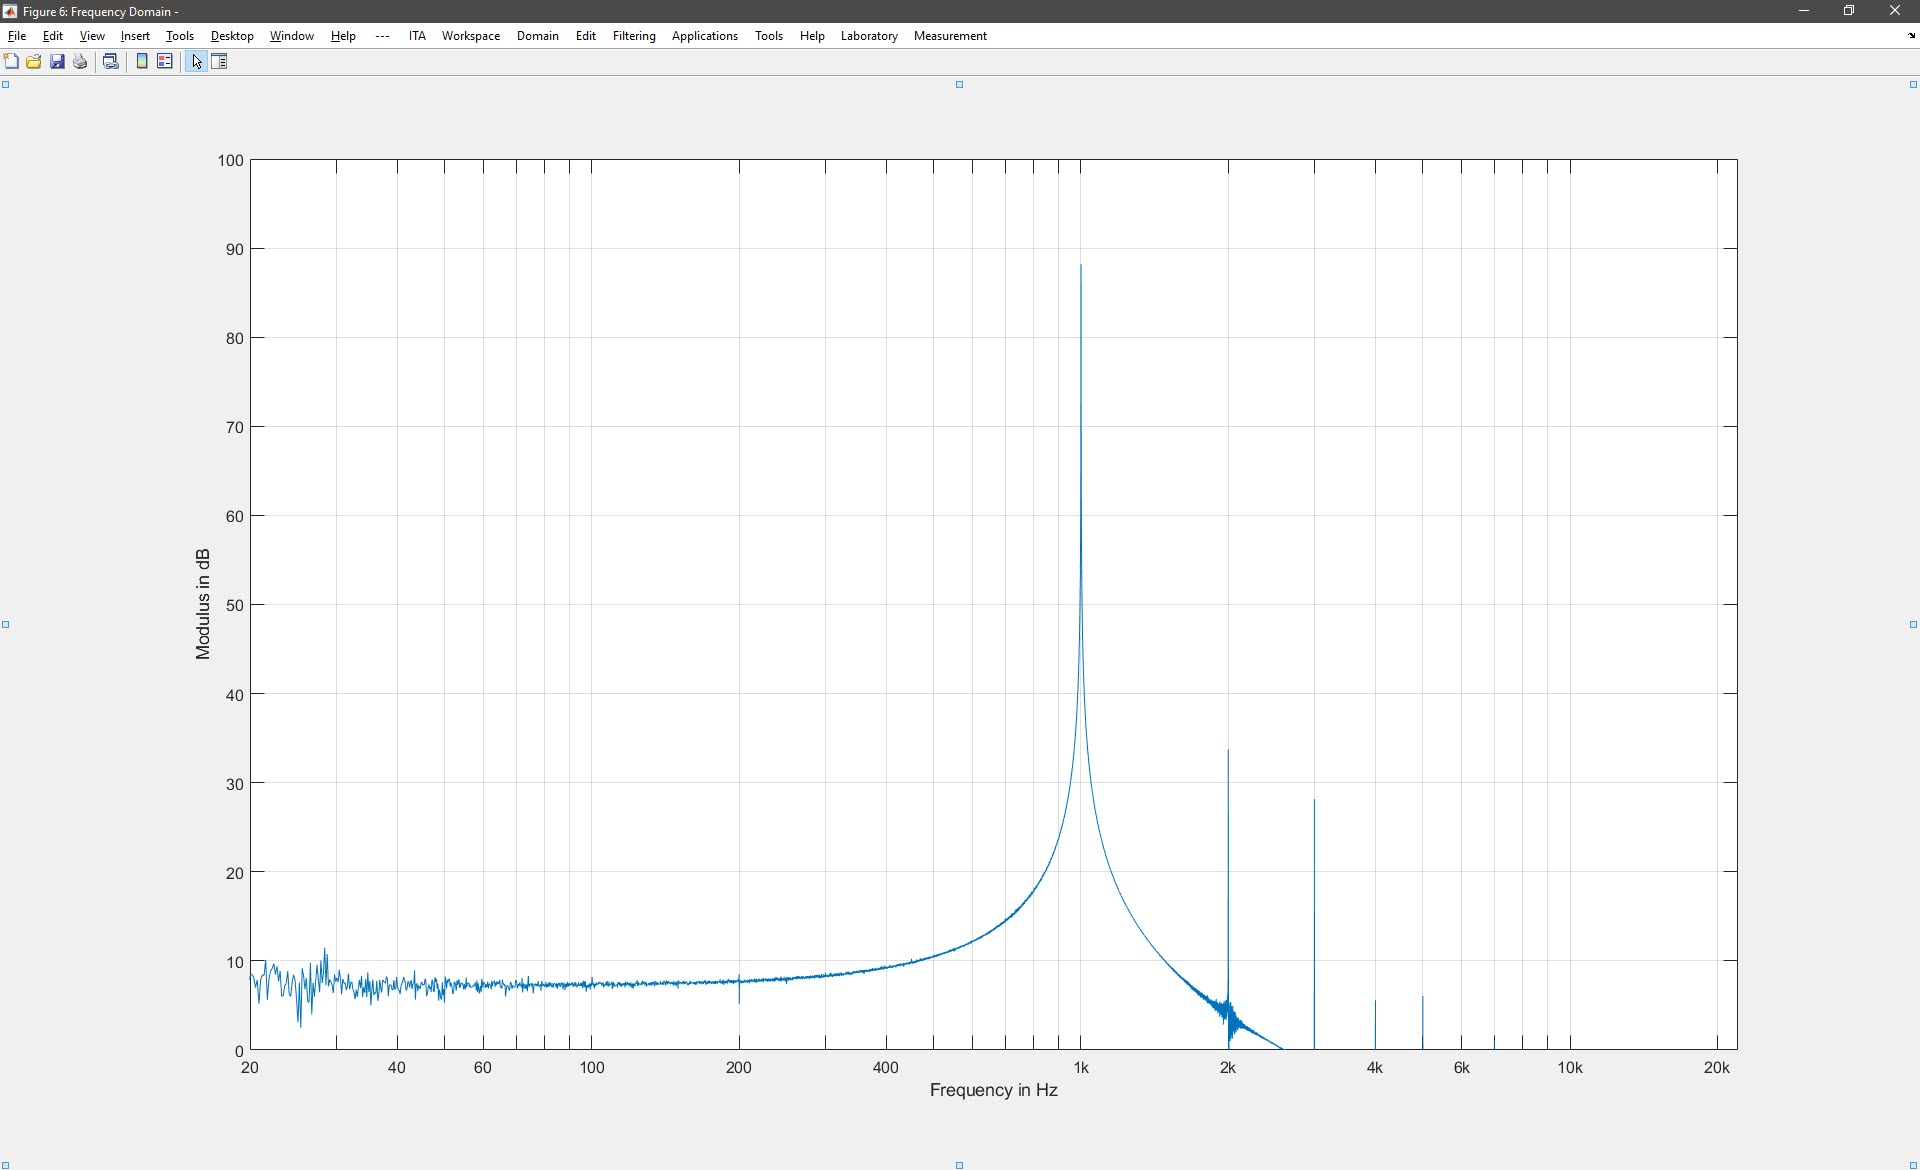
\includegraphics[width=.7\textwidth]{Figures/E15.jpg}
\end{figure}
%%%%%%%%%%%%%%%%%%%%%%%%%%%%%%%%%%%%%%%%%%%%%%%%%%%%%%%%%%%%%%%

%%%%%%%%%%%%%%%%%%%%%%%%%%%%%%%%%%%%%%%%%%%%%%%%%%%%%%%%%%%%%%%
\begin{matlabbox}
%% Calculate correction factor (value [Pa] * factor [Pa] = 10 [Pa])

rightFactor = 10/abs(sampleRecord1kHZ_RIGHT.freq(5948)); %get the value at 1k (pos 5948) factor at 1kHz 
leftFactor = 10/abs(sampleRecord1kHZ_LEFT.freq(5948));   %Pa factor at 1kHz

%% Apply directly to the Right side 
ita_plot_freq((sampleRecord1kHZ_RIGHT*rightFactor)/2e-5)

\end{matlabbox}
\begin{figure}[H] \centering
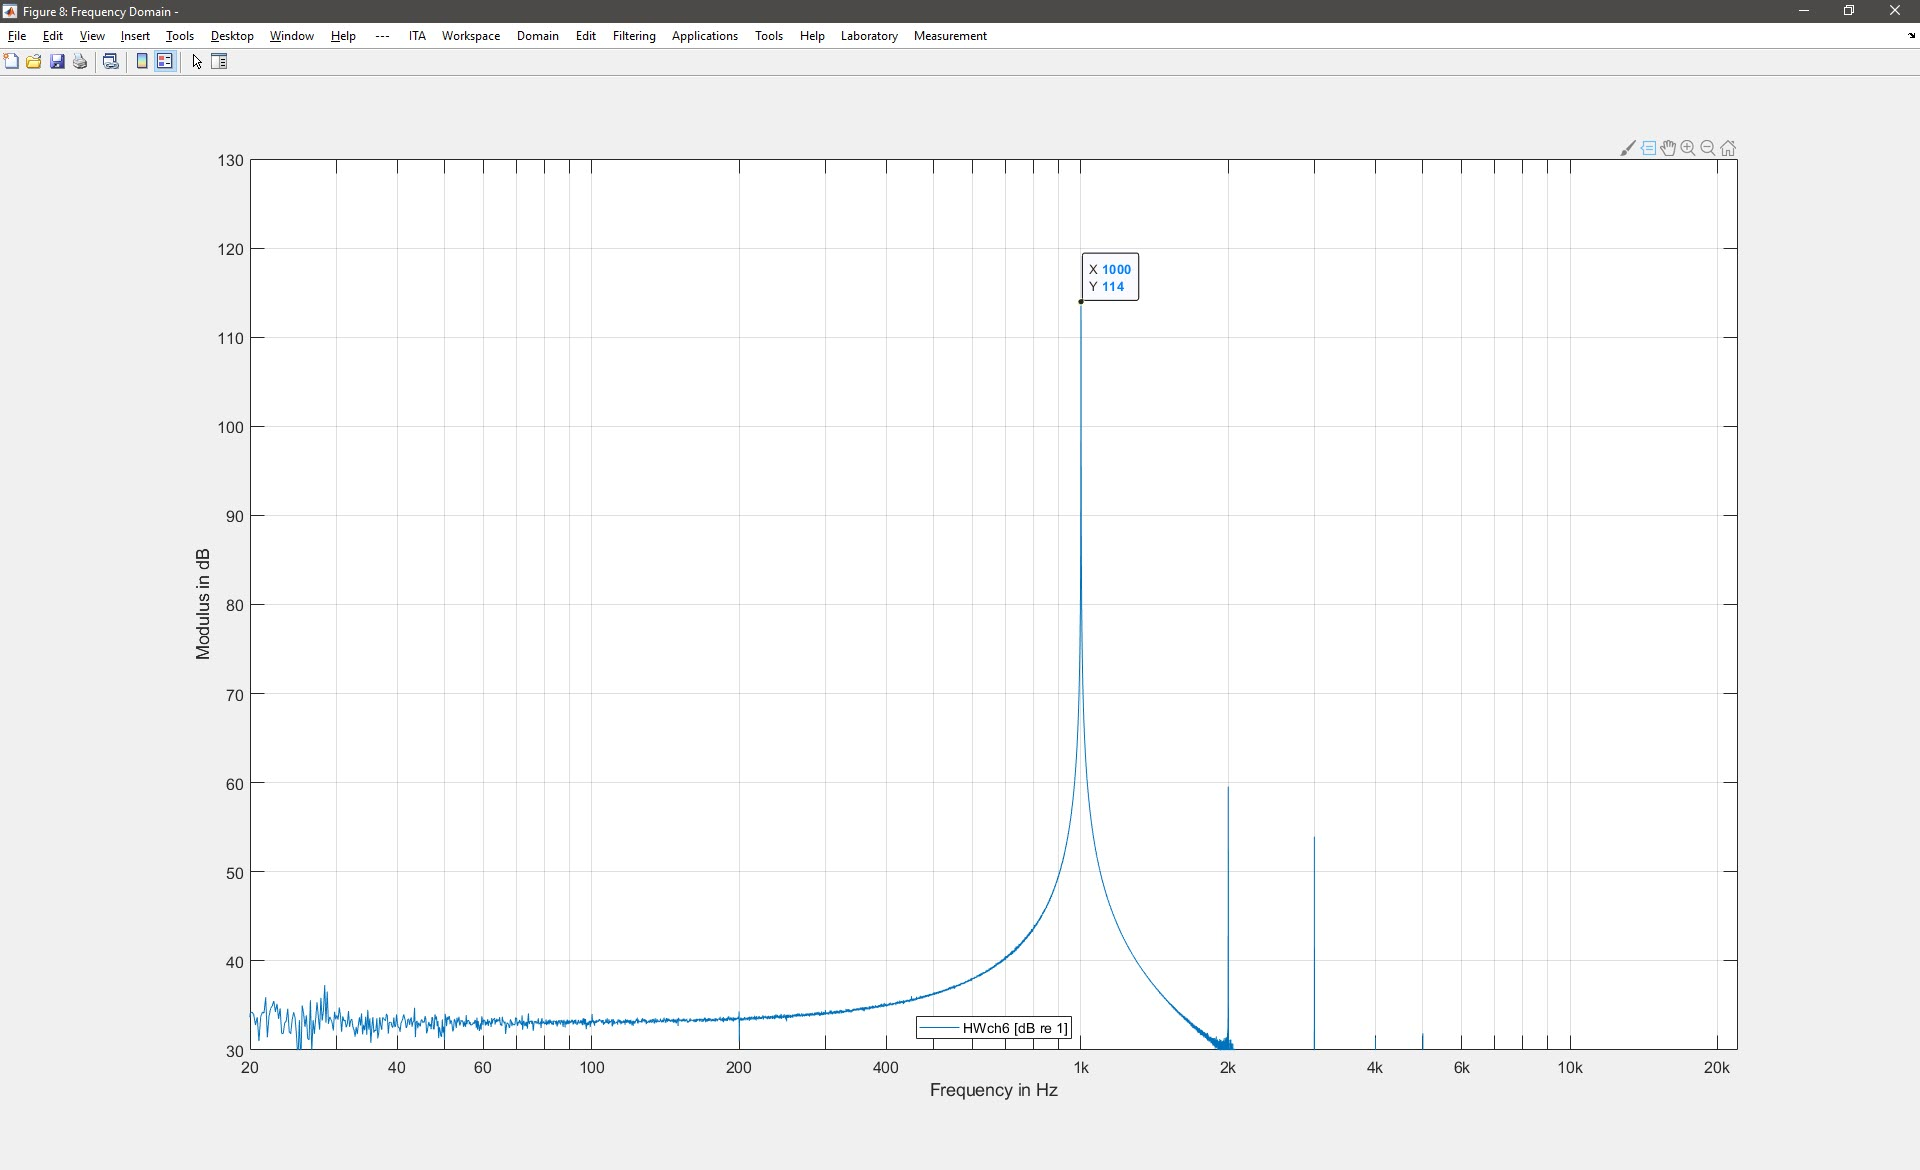
\includegraphics[width=.7\textwidth]{Figures/E16.jpg}
\end{figure}
%%%%%%%%%%%%%%%%%%%%%%%%%%%%%%%%%%%%%%%%%%%%%%%%%%%%%%%%%%%%%%%
\pagebreak
%%%%%%%%%%%%%%%%%%%%%%%%%%%%%%%%%%%%%%%%%%%%%%%%%%%%%%%%%%%%%%%
\begin{matlabbox}
%% or
Simple_rec_right = (sampleRecord1kHZ_RIGHT)/20e-6;
Simple_rec_right.channelUnits = ['20 ' char(181) 'Pa']
Simple_rec_right.channelNames = {'No Correction applied'}

Correct_rec_right = (sampleRecord1kHZ_RIGHT*rightFactor)/20e-6;
Correct_rec_right.channelUnits = ['20 ' char(181) 'Pa']
Correct_rec_right.channelNames = {'Correction applied'}

ita_plot_freq(merge(Simple_rec_right,Correct_rec_right))% 10 Pa appx 114 dB

\end{matlabbox}
\begin{figure}[H] \centering
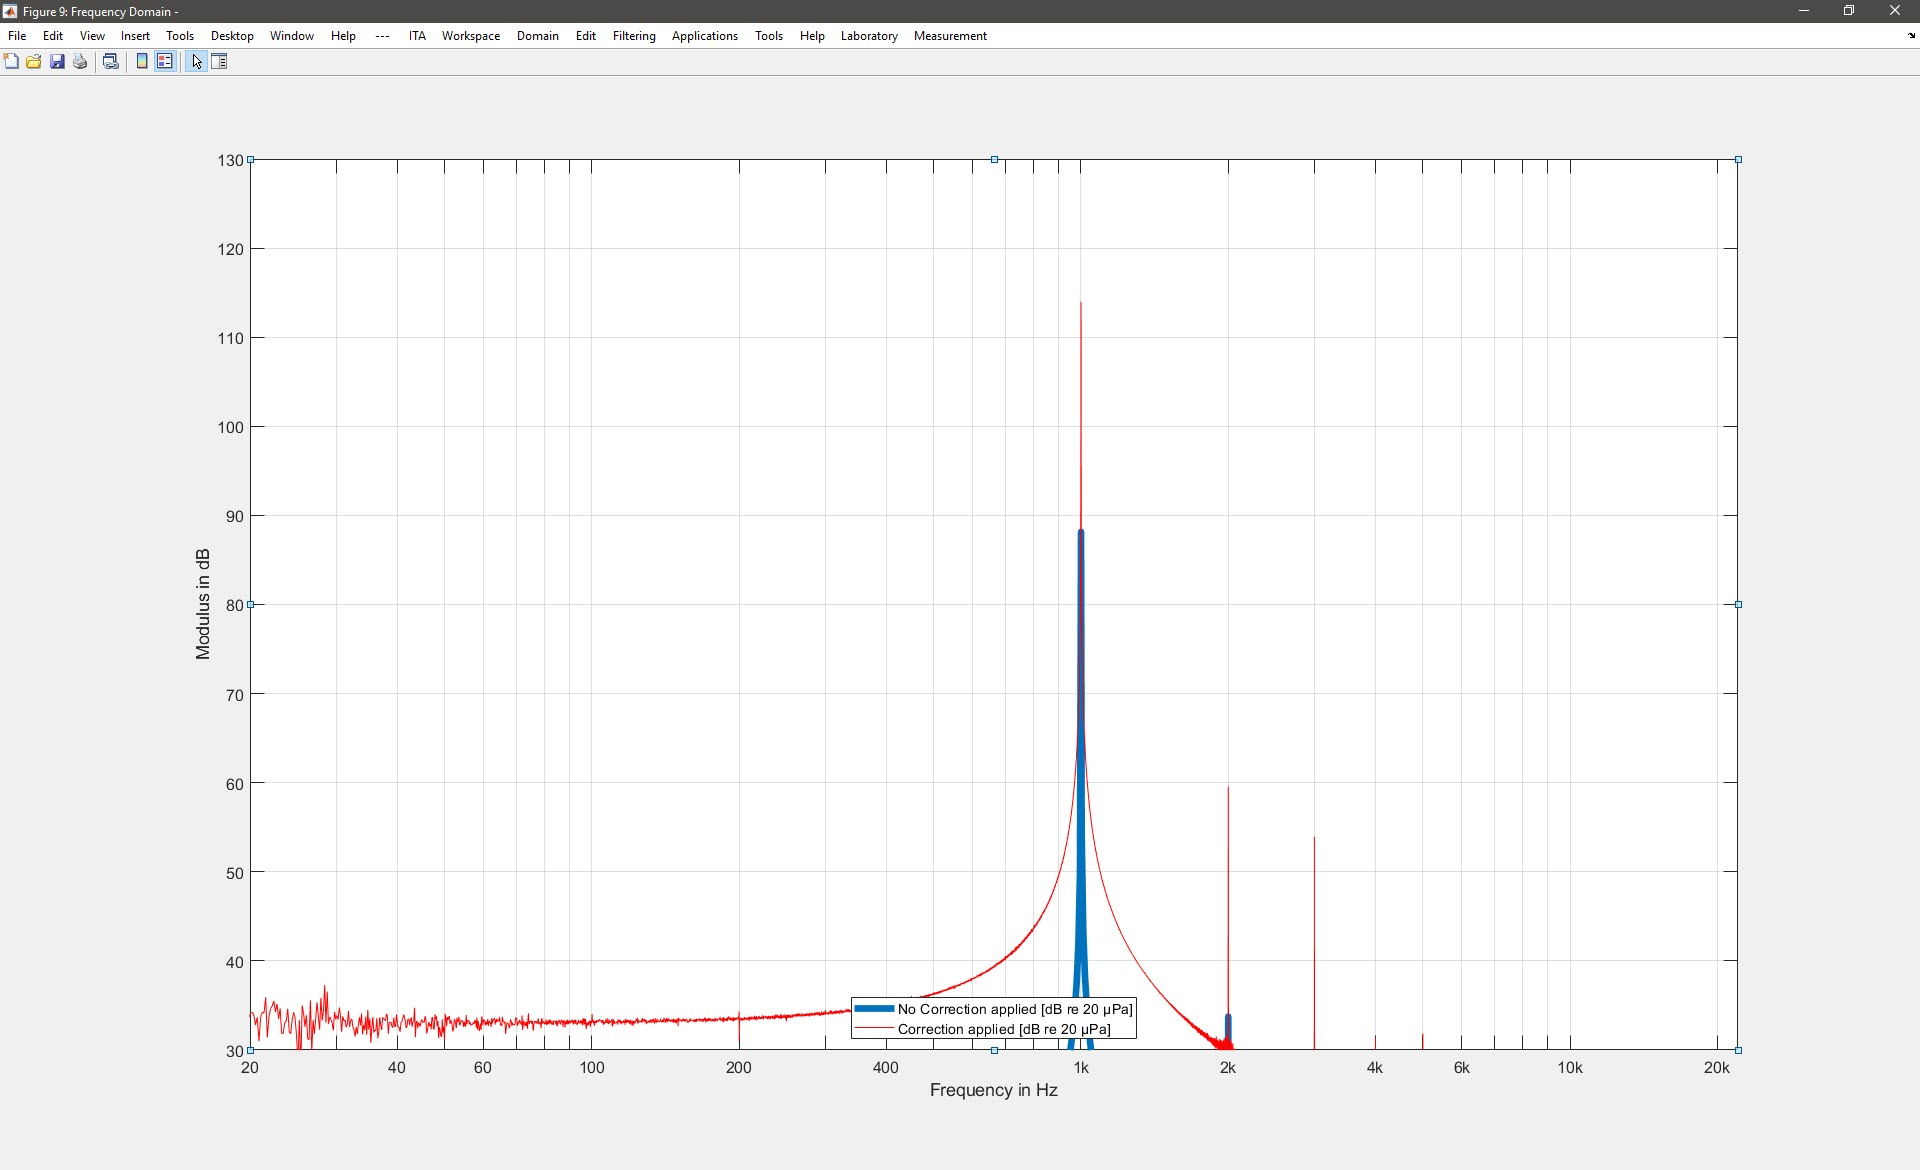
\includegraphics[width=.7\textwidth]{Figures/E17.jpg}
\end{figure}
%%%%%%%%%%%%%%%%%%%%%%%%%%%%%%%%%%%%%%%%%%%%%%%%%%%%%%%%%%%%%%%
%%%%%%%%%%%%%%%%%%%%%%%%%%%%%%%%%%%%%%%%%%%%%%%%%%%%%%%%%%%%%%%
\begin{matlabbox}
%%
L_00= L_00*leftFactor;
L_90= L_90*leftFactor;

R_00= R_00*rightFactor;
R_90= R_90*rightFactor;

%%
FRF_00_Smooth_cropped = ita_merge(L_00,R_00);% Merge to same itaAudio
FRF_90_Smooth_cropped = ita_merge(L_90,R_90);% Merge to same itaAudio

%%
FRF_00_Smooth_cropped.plot_freq

\end{matlabbox}

\begin{figure}[H] \centering
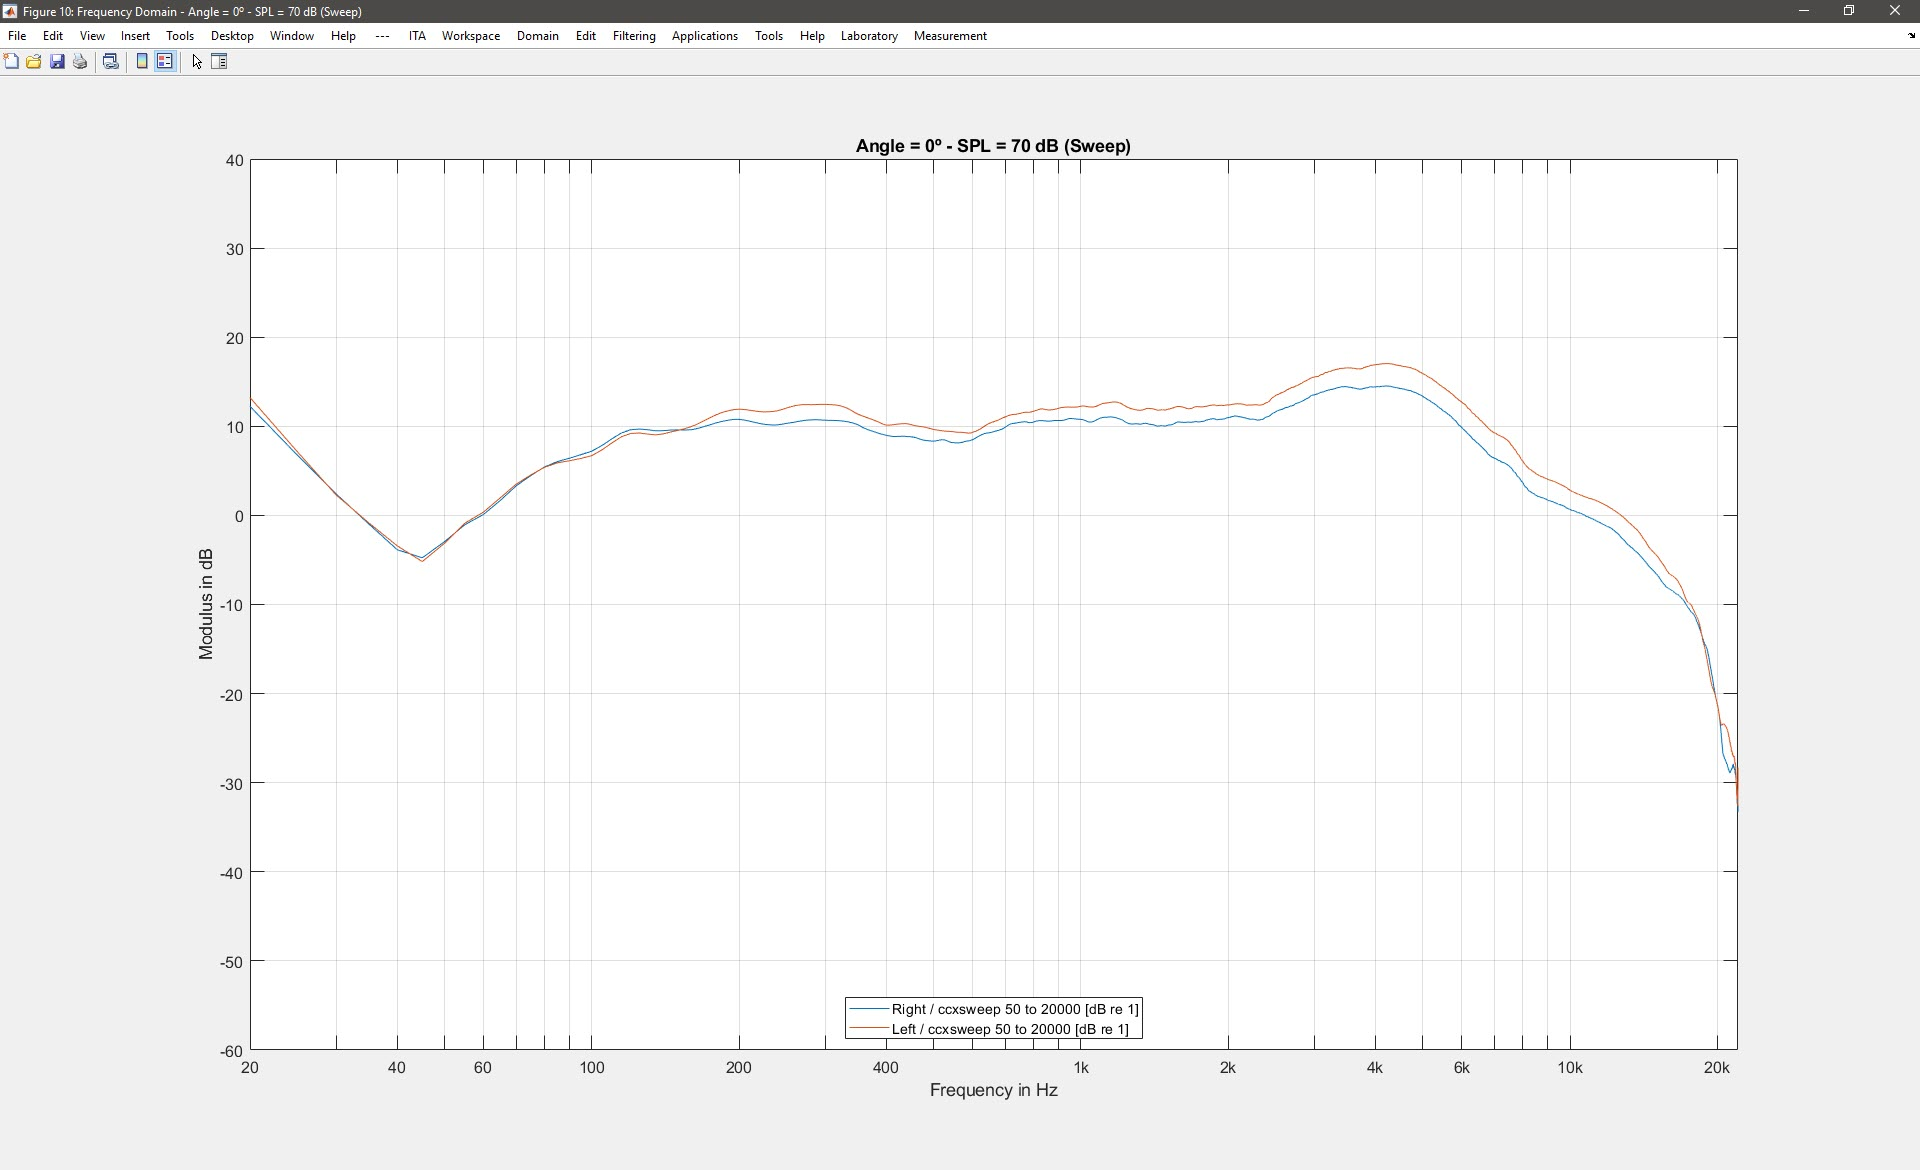
\includegraphics[width=.7\textwidth]{Figures/E18.jpg}
\end{figure}
%%%%%%%%%%%%%%%%%%%%%%%%%%%%%%%%%%%%%%%%%%%%%%%%%%%%%%%%%%%%%%%
%%%%%%%%%%%%%%%%%%%%%%%%%%%%%%%%%%%%%%%%%%%%%%%%%%%%%%%%%%%%%%%
\begin{matlabbox}
%%

FRF_Filter_00 = ita_filter_bandpass(FRF_00_Smooth_cropped,'lower', 200, 'upper', 5000);  %filter 50 to 20k
FRF_Filter_90 = ita_filter_bandpass(FRF_90_Smooth_cropped,'lower', 200, 'upper', 5000);  

%%
FRF_Filter_90.plot_freq_freq

\end{matlabbox}

\begin{figure}[H] \centering
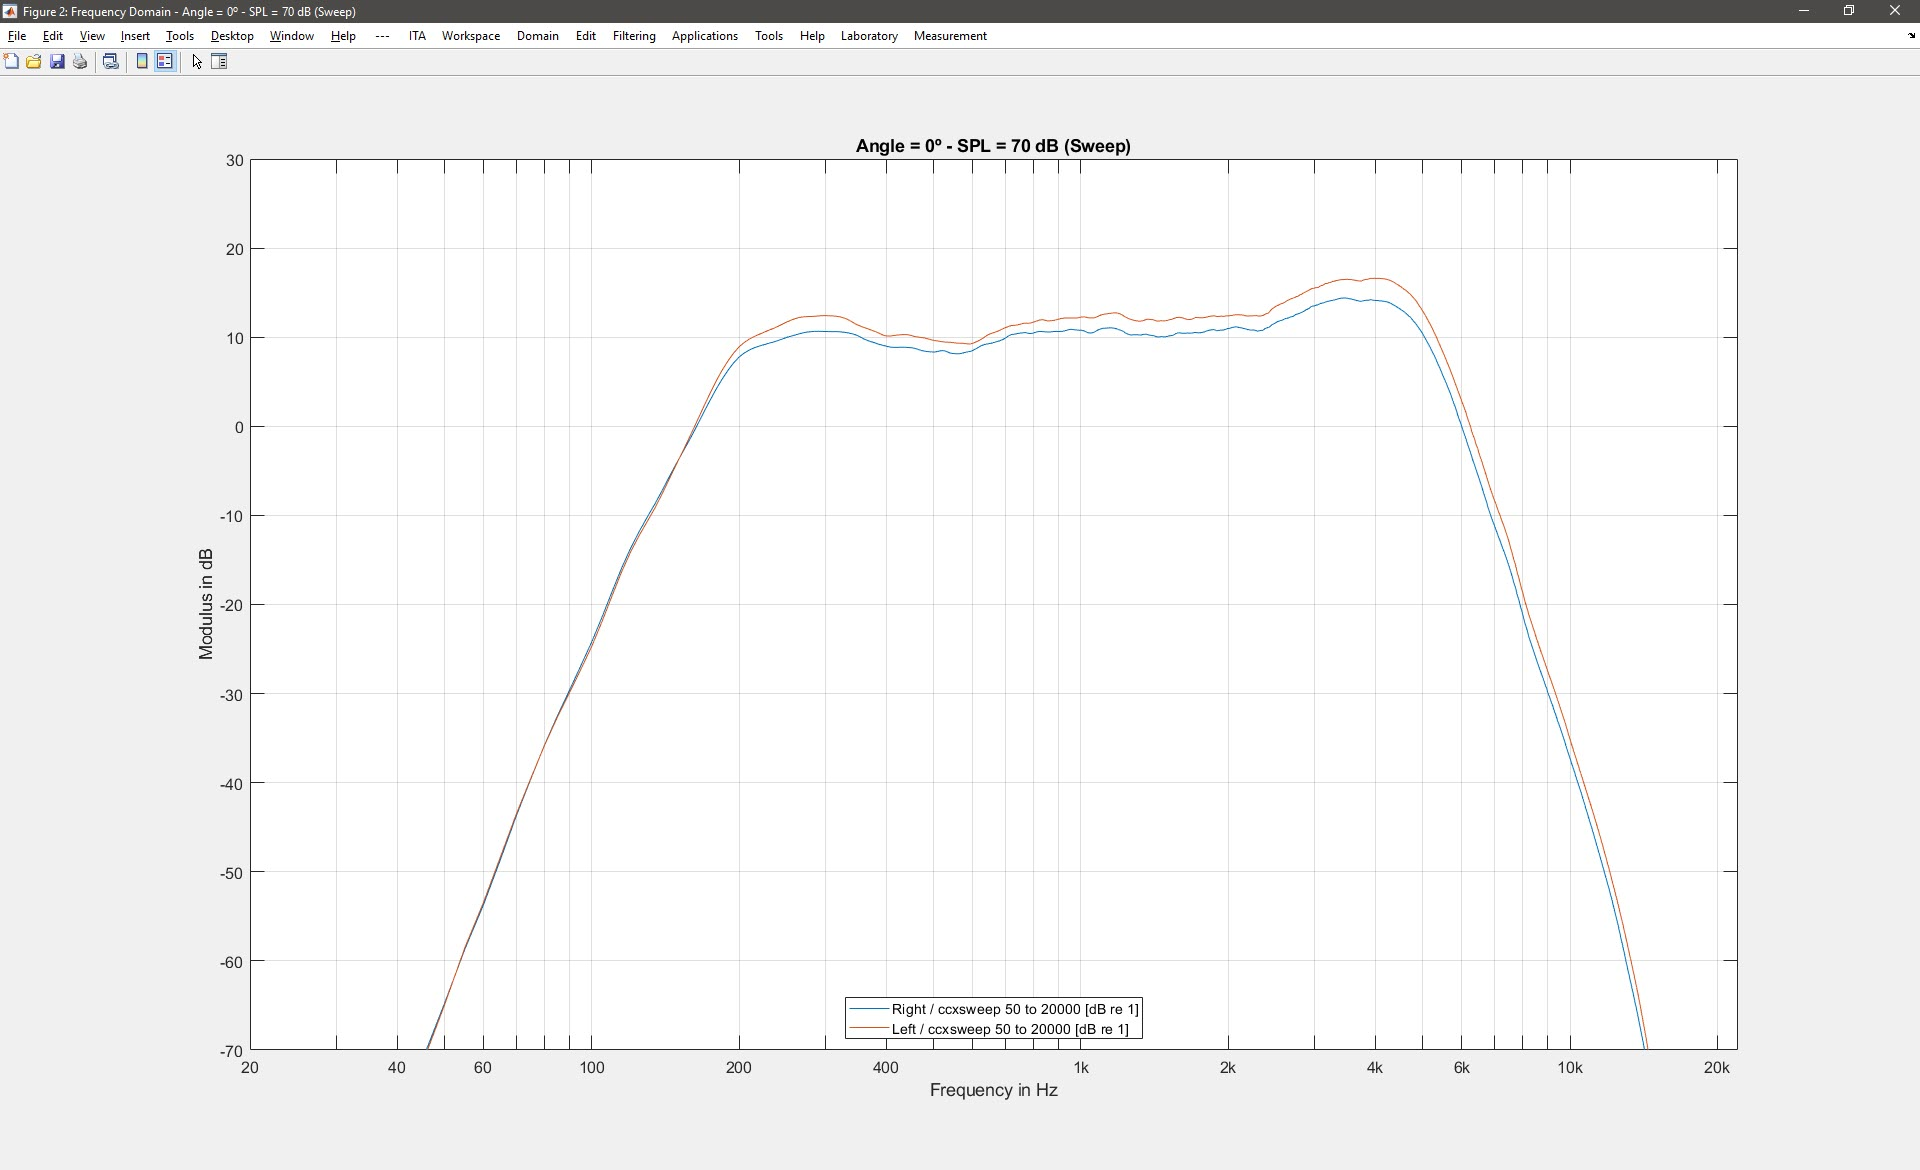
\includegraphics[width=.7\textwidth]{Figures/E19.jpg}
\end{figure}
%%%%%%%%%%%%%%%%%%%%%%%%%%%%%%%%%%%%%%%%%%%%%%%%%%%%%%%%%%%%%%%
%%%%%%%%%%%%%%%%%%%%%%%%%%%%%%%%%%%%%%%%%%%%%%%%%%%%%%%%%%%%%%%
\begin{matlabbox}
%% plot Bar
FRF_third_octave_00.bar

\end{matlabbox}

%%%%%%%%%%%%%%%%%%%%%%%%%%%%
\begin{figure}[H] \centering
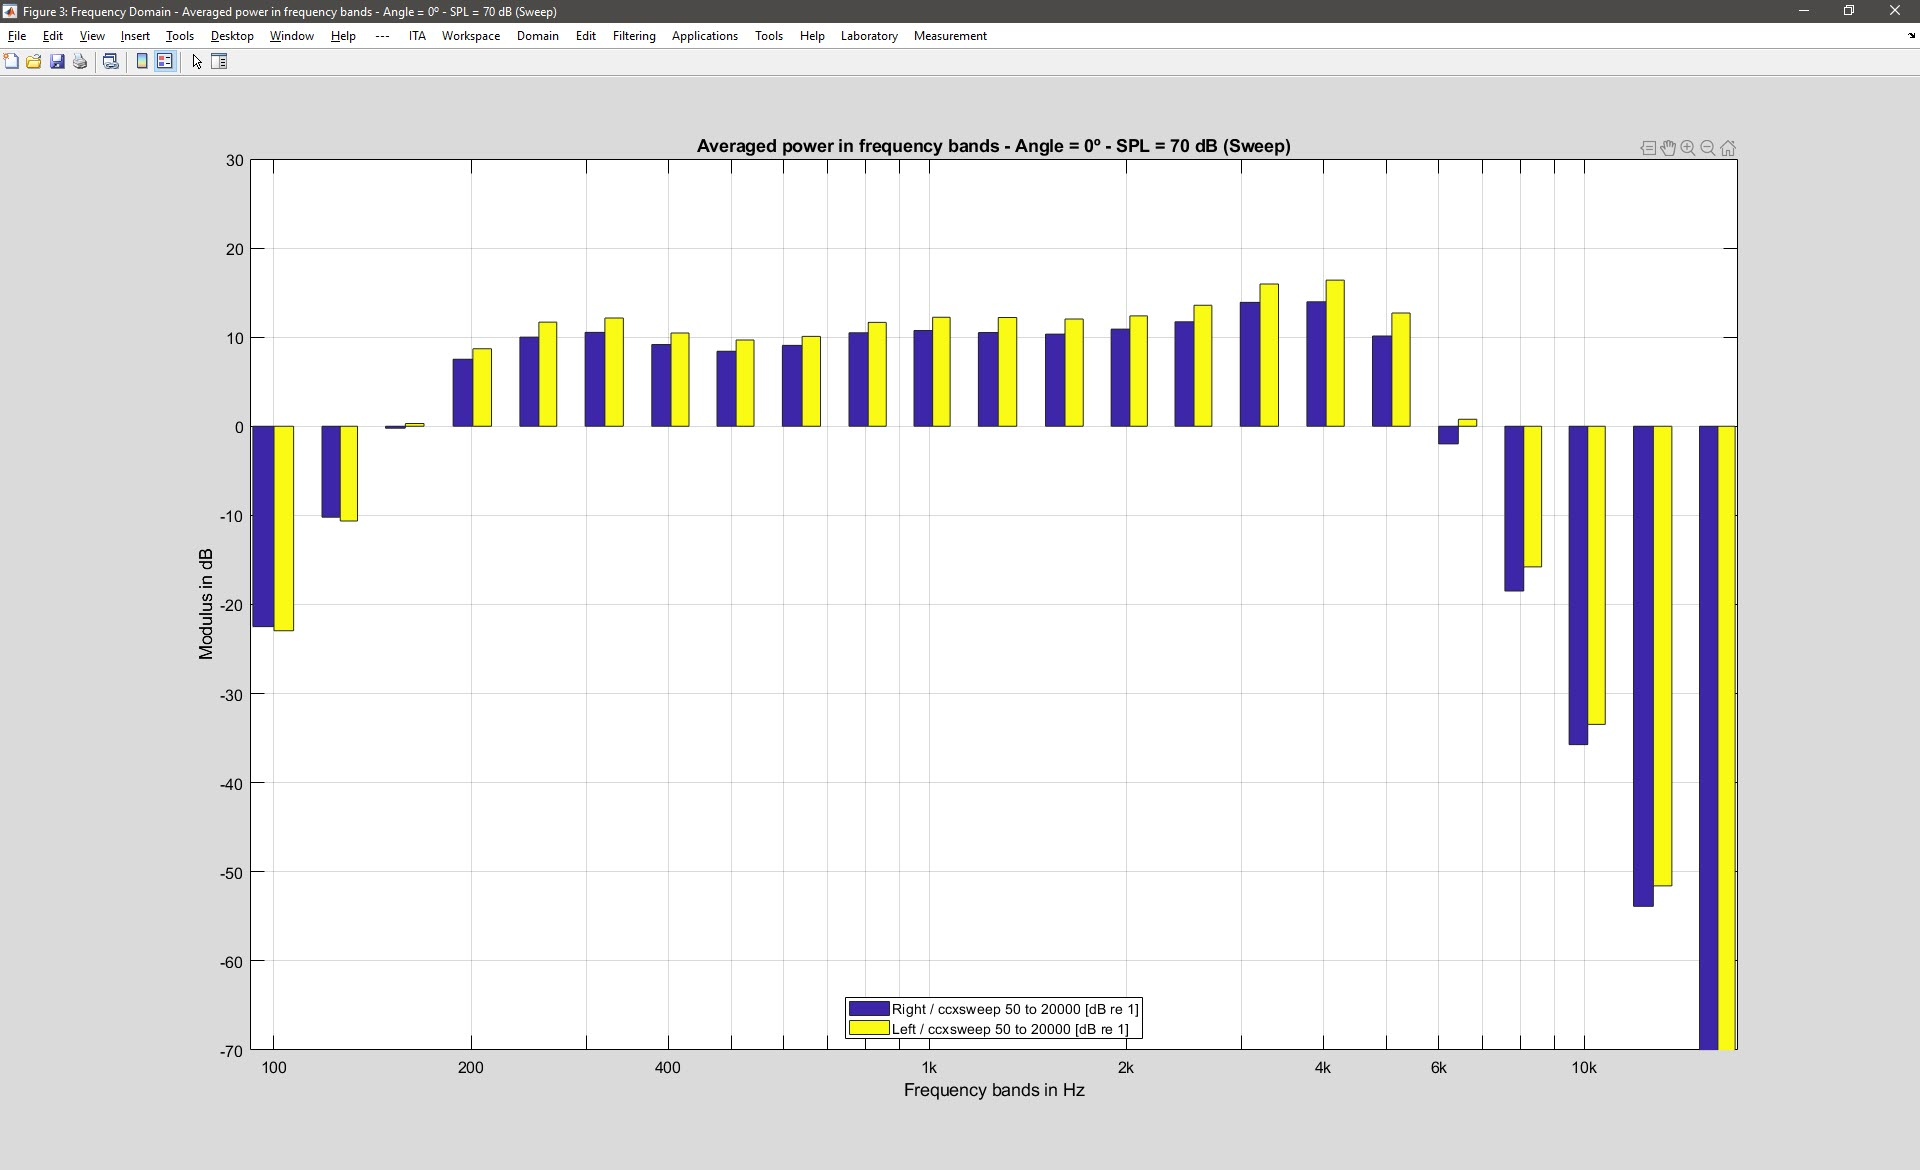
\includegraphics[width=.7\textwidth]{Figures/E20.jpg}
\end{figure}
%%%%%%%%%%%%%%%%%%%%%%%%%%%%

\pagebreak
%%%%%%%%%%%%%%%%%%%%%%%%%%%%%%%%%%%%%%%%%%%%%%%%%%%%%%%%%%%%%%%
%%%%%%%%%%%%%%%%%%%%%%%%%%%%%%%%%%%%%%%%%%%%%%%%%%%%%%%%%%%%%%%
\begin{matlabbox}
%% Plot Line
ita_plot_freq(FRF_third_octave_00)
\end{matlabbox}

%%%%%%%%%%%%%%%%%%%%%%%%%%%%
\begin{figure}[H] \centering
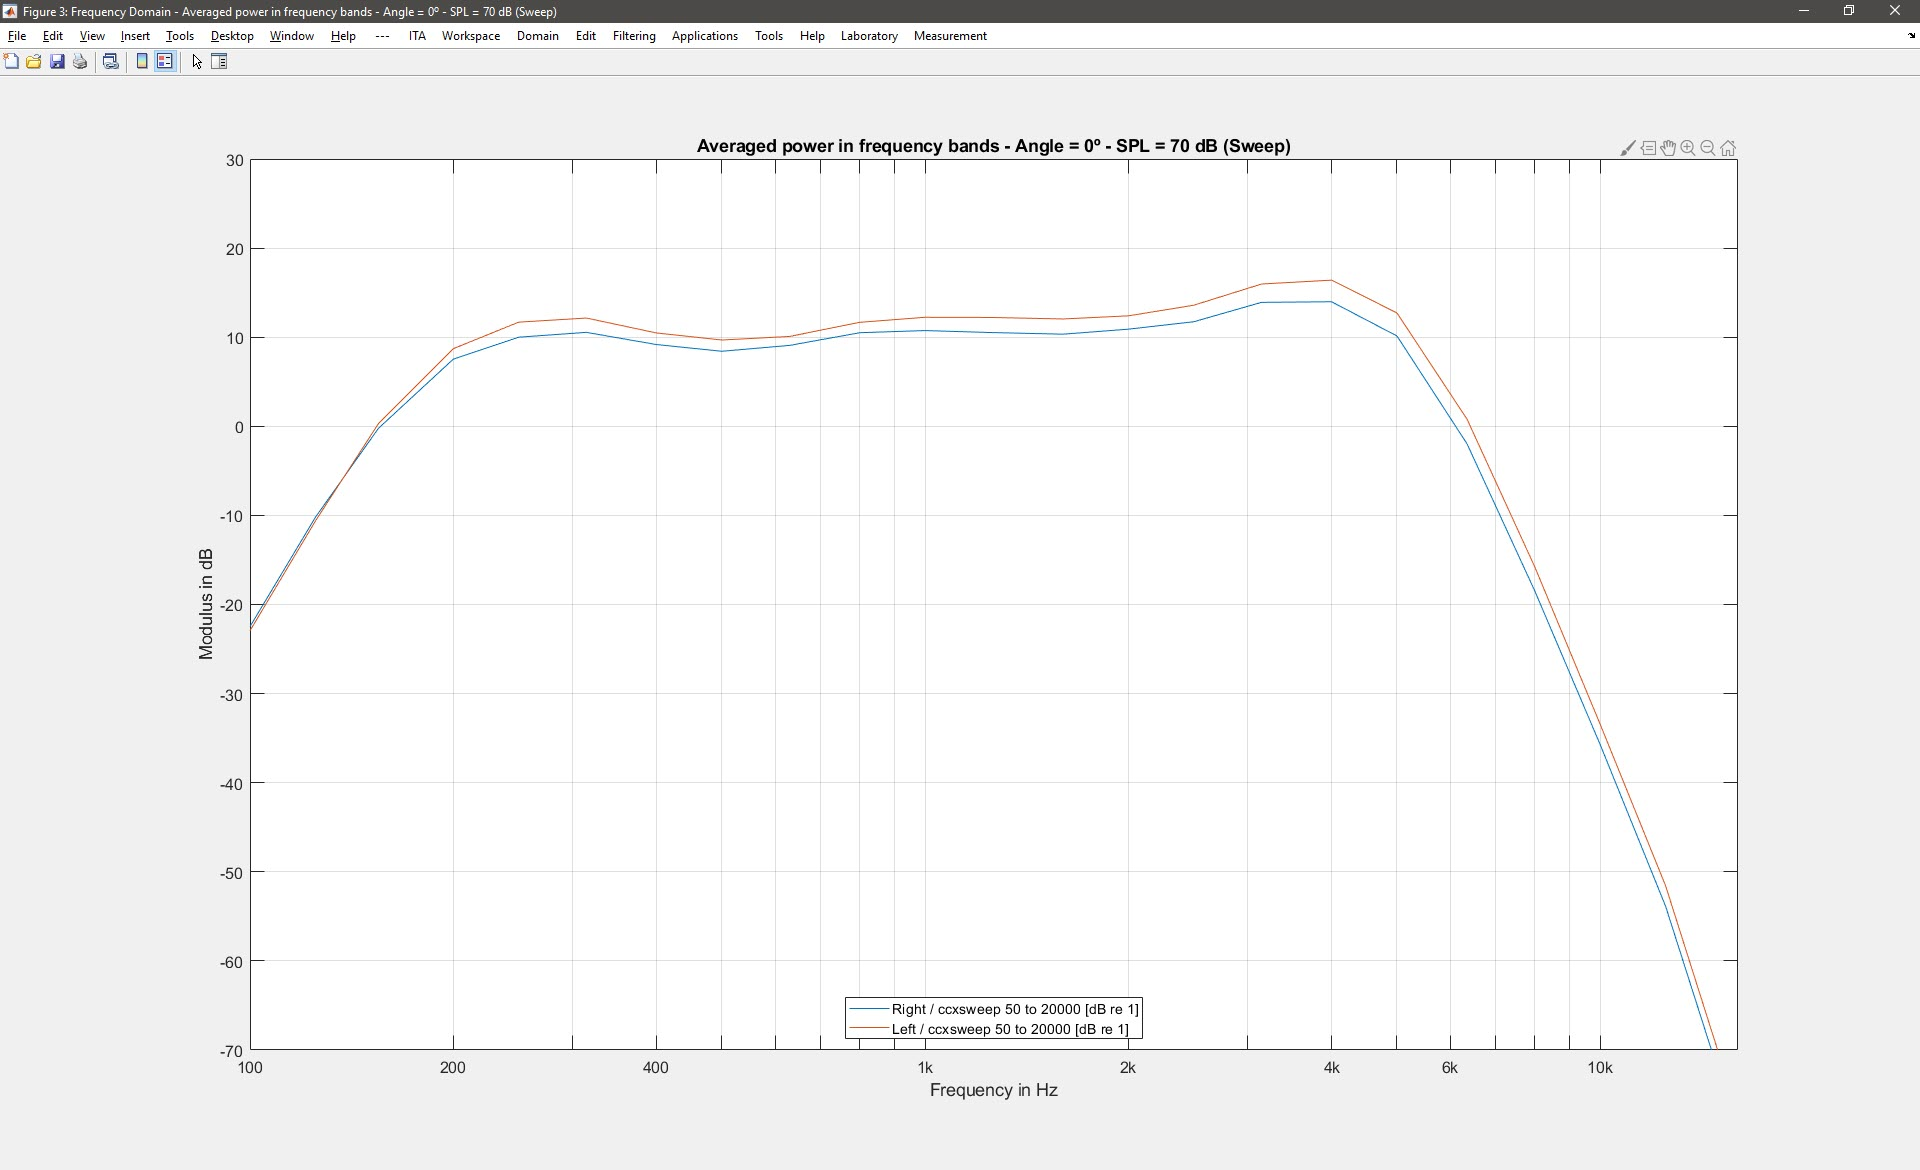
\includegraphics[width=.7\textwidth]{Figures/E21.jpg}
\end{figure}
%%%%%%%%%%%%%%%%%%%%%%%%%%%%

%%%%%%%%%%%%%%%%%%%%%%%%%%%%%%%%%%%%%%%%%%%%%%%%%%%%%%%%%%%%%%%
%%%%%%%%%%%%%%%%%%%%%%%%%%%%%%%%%%%%%%%%%%%%%%%%%%%%%%%%%%%%%%%
\begin{matlabbox}
%% Measurement
%you can call a GUI and configure everything
m = ita_measurement
\end{matlabbox}

%%%%%%%%%%%%%%%%%%%%%%%%%%%%
\begin{figure}[H] \centering
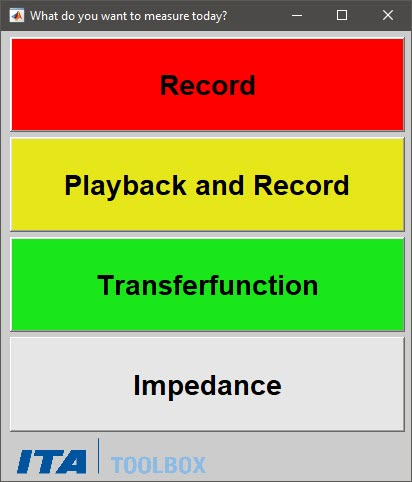
\includegraphics[width=.4\textwidth]{Figures/E22.jpg}
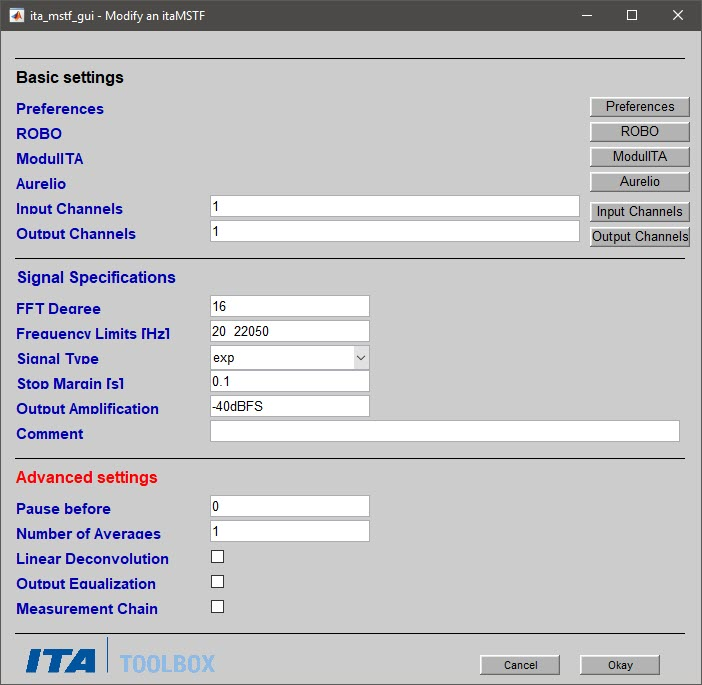
\includegraphics[width=.5\textwidth]{Figures/E23.jpg}
\end{figure}
%%%%%%%%%%%%%%%%%%%%%%%%%%%%
%%%%%%%%%%%%%%%%%%%%%%%%%%%%%%%%%%%%%%%%%%%%%%%%%%%%%%%%%%%%%%%
\pagebreak
%%%%%%%%%%%%%%%%%%%%%%%%%%%%%%%%%%%%%%%%%%%%%%%%%%%%%%%%%%%%%%%
\begin{matlabbox}
%% Or create in a quick way
MS = itaMSTF
MS.edit
%% or set
inputChannels = 1:29
trackLength   = 4;            % length of excitation signal in seconds
type          = 'exp';        % type of excitation signal: exponential sweep
freqRange     = [20,12000];   % frequency range of sweep
stopMargin    = 0.1;          % the last part of the excitation is silent to allow all frequencies to decay
averages      = 1;            % number of averages
commentStr    = 'Example measurement 2014-11-27';

inputChannels      = 1:3;
outputChannels     = 1;

outputamplification = -35;    % Digital output amplification in dBFS. 0 dBFS is maximum. This amplification is automatically compensated in the measurement.

useMeasurementChain = false;  % measurement chain is needed for calibration
pauseTime           = 0;      % time in seconds pause before measurement
%% good way

MS = itaMSTF('freqRange', freqRange, 'trackLength', trackLength, 'stopMargin', stopMargin, ...
    'inputChannels', inputChannels, 'outputChannels', outputChannels, 'averages', averages, ...
    'pause' , pauseTime, 'comment', commentStr, 'type', type, 'outputamplification', outputamplification, ...
    'useMeasurementChain', useMeasurementChain);
    
    %% Configured...
    %% run
MS.run
% this method records background noise and raw signal and calculates the
% signal to noise ratio in frequency bands
snr = MS.run_snr;
snr.plot_freq

\end{matlabbox}
You can use the same idea to the itaMSRecord, itaMSPlaybackRecord and others measurements.

%%%%%%%%%%%%%%%%%%%%%%%%%%%%%%%%%%%%%%%%%%%%%%%%%%%%%%%%%%%%%%%
%%%%%%%%%%%%%%%%%%%%%%%%%%%%%%%%%%%%%%%%%%%%%%%%%%%%%%%%%%%%%%%
\begin{matlabbox}
%% a little of room acoustics
%open GUI
ita_roomacoustics
%%
RA_param = ita_roomacoustics(L_00)
%% Direct
RA_param = ita_roomacoustics(L_00,'freqRange', [100 4000], 'bandsPerOctave', 1,'T30', 'T20', 'T30', 'T40', 'C50', 'C80','EDT') 
%% itaResult 
%Plot the T20 result (same applies to all parameters)
RA_param.T20.bar
%%
frequency_vector = RA_param.T20.freqData
\end{matlabbox}

%%%%%%%%%%%%%%%%%%%%%%%%%%%%%%%%%%%%%%%%%%%%%%%%%%%%%%%%%%%%%%%
%%%%%%%%%%%%%%%%%%%%%%%%%%%%%%%%%%%%%%%%%%%%%%%%%%%%%%%%%%%%%%%


\end{document}

